\documentclass[11pt,a4paper]{article}
\usepackage[utf8]{inputenc}
\usepackage[T1]{fontenc}
\usepackage{amsmath,amssymb,amsthm}
\usepackage{bbm}
\usepackage{geometry}
\usepackage{braket}
\usepackage{tikz}
\geometry{margin=2.5cm}
\usepackage{hyperref}

\newcommand{\op}[1]{\hat{#1}}
\newcommand{\ud}{\mathrm{d}}

\title{NJSF064 --- Nuclear Physics\\[2mm]\large Block 1: Deuteron and nucleon-nucleon interaction}
\author{František Knapp}
\date{}

\begin{document}
\maketitle

%\tableofcontents

%=====================================================================
\section{Isospin in nuclear physics (isobaric spin)}
%=====================================================================
Proton and neutron have similar masses and behave similarly with respect to the strong interaction. In nuclear physics context, therefore, it is sometimes convenient to think in terms of a single particle, the "nucleon", and to consider the proton and the neutron as two states of the "nucleon". Mathematical analogy to the spin formalism leads us to the introduction of iso(topic) spin.

\[
\ket{n} \;\longrightarrow\; \begin{pmatrix}1\\0\end{pmatrix},
\qquad \text{isospin projection } t_z = +\tfrac12 
\]
\[
\ket{p} \;\longrightarrow\; \begin{pmatrix}0\\1\end{pmatrix},
\qquad  \text{isospin projection } t_z = -\tfrac12 
\]
This corresponds to the common convention used in nuclear physics, whereas particle physicists use oposite one (i.e. $t_z = +\tfrac12 $ for the proton and $t_z = -\tfrac12 $  for the neutron)

%\subsection{Isospin operators}
In complete analogy to spin $1/2$ case we can define operators acting in isospin space
\[        
[\op\tau_i,\op\tau_j] = 2i\,\varepsilon_{ijk}\,\op\tau_k ,
\qquad
\{\op\tau_i,\op\tau_j\} = 2\,\delta_{ij}\,\mathbbm{1},
\qquad i=1,2,3 ,
\]
where 
\[
\op\tau_x=\begin{pmatrix}0&1\\1&0\end{pmatrix},\qquad
\op\tau_y=\begin{pmatrix}0&-i\\ i&0\end{pmatrix},\qquad
\op\tau_z=\begin{pmatrix}1&0\\0&-1\end{pmatrix}
\]
are isospin Pauli matrices. 

Isospin operators are given by 
\[
\op t_i = \tfrac12\op\tau_i ,\qquad
[\op t_i,\op t_j] = i\,\varepsilon_{ijk}\,\op t_k ,\qquad
\op t_\pm = \op t_x \pm i\op t_y .
\]
\[
\op t_+=\begin{pmatrix}0&1\\0&0\end{pmatrix},\qquad
\op t_-=\begin{pmatrix}0&0\\1&0\end{pmatrix},
\]
\[
\op t_+\begin{pmatrix}1\\0\end{pmatrix}=0,\quad
\op t_+\begin{pmatrix}0\\1\end{pmatrix}=\begin{pmatrix}1\\0\end{pmatrix}
\quad\Longleftrightarrow\quad \op t_+\ket{n}=0 , \quad \op t_+\ket{p}=\ket{n},
\]
\[
\op t_-\begin{pmatrix}1\\0\end{pmatrix}=\begin{pmatrix}0\\1\end{pmatrix},\quad
\op t_-\begin{pmatrix}0\\1\end{pmatrix}=0
\quad\Longleftrightarrow\quad \op t_-\ket{n}=\ket{p}, \quad \op t_-\ket{p}= 0.
\]

%\subsection{Many-nucleon isospin}

We can generalize isospin for a many-nucleon system composed of $A$ nucleons:
\[
\op{\vec T}=\sum_{i=1}^A \op{\vec t}^{(i)} ,\qquad
\op {\vec T}^2=\op T_x^2+\op T_y^2+\op T_z^2,\qquad
\op T_z=\sum_{i=1}^{A}\op t_z^{(i)}.
\]
One can construct states with total isospin $T$ and projection $T_z$, labeled
$T_z,\,T$.

For a nuclear state $\ket{N,Z}$ with $N$ neutrons and $Z$ protons, the isospin
projection is
\[
\op T_z\ket{N,Z}=\sum_i \op t_z^{(i)}\ket{N,Z}=\tfrac12(N-Z)\,\ket{N,Z},
\]
because
\[
\ket{N,Z}=\big|\, t_z^{(1)},t_z^{(2)},t_z^{(3)},\dots,t_z^{(A)}\,\big\rangle,
\qquad t_z^{(i)}=\pm\tfrac12 .
\]
Therefore, if $N=Z$, then $T_z=0$.

Similarly to angular momentum, $T_z\in\{-T,-T+1,\dots,T-1,T\}$. For $N=Z$,
$T_z=0$ is the only allowed value; if there is only one $T_z=0$ state $\Rightarrow
T=0$. In general, for $N\ne Z$,
\[
T_z=\tfrac12(N-Z),\qquad T\ge |T_z| .
\]
Eigenstates of Hamiltonian with good isospin can be constructed if the Hamiltonian is isospin invariant, i.e.  
\[
[\op H,\op {\vec T}^2]=0,\qquad [\op H,\op T_z]=0, 
\]
\[
\op H \ket{T T_z} = E \ket{T T_z} 
\]
\[
\op T^2\ket{T T_z}=T(T+1)\ket{T T_z}
\]
\[
\op T_z\ket{T T_z }=T_z\ket{T  T_z}.
\]
in complete analogy to total angular momentum. 
However, contrary to rotational invariance of nuclear Hamiltonian, isospin invariance is not exact symmetry. In fact, the Coulomb interaction violates isospin symmetry. It turns out that inspite of this obvious violation it still useful in many cases to label states according to $T$.
\\
\par 
Let us assume explicitly the 2-nucleon case, with $\op{\vec t}^{(1)},\op{\vec t}^{(2)}$:
\[
\big|t^{(1)}t^{(2)},T\,T_z\big\rangle=
\sum_{t_z^{(1)},t_z^{(2)}}
\big(t^{(1)}t_z^{(1)}\,t^{(2)}t_z^{(2)}\,\big|\,T\,T_z\big)\,
\big|t^{(1)}t_z^{(1)}\big\rangle^{(1)}\big|t^{(2)}t_z^{(2)}\big\rangle^{(2)},
\qquad t^{(1)}=t^{(2)}=\tfrac12 .
\]
We can construct isospin singlet \\
$T=0,\ T_z=0$:
\[
\big|\tfrac12\tfrac12,00\big\rangle
=\frac{1}{\sqrt2}\Big\{\big|\tfrac12\tfrac12\big\rangle^{(1)}\big|\tfrac12{-}\tfrac12\big\rangle^{(2)}
-\big|\tfrac12{-}\tfrac12\big\rangle^{(1)}\big|\tfrac12\tfrac12\big\rangle^{(2)}\Big\}
\;\Longleftrightarrow\;
\frac{1}{\sqrt2}\big\{\ket{n}^{(1)}\ket{p}^{(2)}-\ket{p}^{(1)}\ket{n}^{(2)}\big\}.
\]
and isospin triplet \\
$T=1,\ T_z=0$:
\[
\big|\tfrac12\tfrac12,10\big\rangle
=\frac{1}{\sqrt2}\Big\{\big|\tfrac12\tfrac12\big\rangle^{(1)}\big|\tfrac12{-}\tfrac12\big\rangle^{(2)}
+\big|\tfrac12{-}\tfrac12\big\rangle^{(1)}\big|\tfrac12\tfrac12\big\rangle^{(2)}\Big\}
\;\Longleftrightarrow\;
\frac{1}{\sqrt2}\big\{\ket{n}^{(1)}\ket{p}^{(2)}+\ket{p}^{(1)}\ket{n}^{(2)}\big\}.
\]
$T=1,\ T_z=1$: \\
\[
\big|\tfrac12\tfrac12,11\big\rangle=\big|\tfrac12\tfrac12\big\rangle^{(1)}\big|\tfrac12\tfrac12\big\rangle^{(2)}
\;\Longleftrightarrow\;
\ket n^{(1)}\ket n^{(2)}
\]
\\
$T=1,\ T_z=-1$:\\
\[
\big|\tfrac12\tfrac12,1{-}1\big\rangle=\big|\tfrac12{-}\tfrac12\big\rangle^{(1)}\big|\tfrac12{-}\tfrac12\big\rangle^{(2)}
\;\Longleftrightarrow\; \ket p^{(1)}\ket p^{(2)}.
\]
For many-nucleon system for the operator of the total isospin we have 
\[
\op {\vec T}^2=\Big(\sum_{i=1}^A\op{\vec t}^{(i)}\Big)^2
=\big(\op{\vec t}^{(1)}+\op{\vec t}^{(2)}+\dots+\op{\vec t}^{(A)}\big)^2
=\sum_{i=1}^A \op{\vec t}^{(i)2}+2\!\!\sum_{\substack{i<j\\ i=1..A,\;j=1..A}}\!\!\op{\vec t}^{(i)}\!\cdot\op{\vec t}^{(j)} .
\]

Let us define an operator 
\[
\op P_{ij}=\tfrac12\big(\mathbbm{1}+\op{\vec\tau}^{(i)}\!\cdot\op{\vec\tau}^{(j)}\big)
=\tfrac12 \mathbbm{1}+2\,\op{\vec t}^{(i)}\!\cdot\op{\vec t}^{(j)}.
\]
Then
\[
\op {\vec T}^2=\sum_{i=1}^A \op{\vec t}^{(i)2}+\sum_{i<j}\big(\op P_{ij}-\tfrac12 \mathbbm{1}\big) .
\]
One can observe that $\op P_{ij}$ is the isospin exchange operator (it exchanges the isospin projections of the $i$-th and $j$-th nucleon; see below).
For any two nucleons we can show via direct computation, e.g. by explicit use of Pauli matrices following relations
\[
\op P_{ij}\ket n^{(i)}\ket n^{(j)}=\ket n^{(i)}\ket n^{(j)},\qquad
\op P_{ij}\ket p^{(i)}\ket n^{(j)}=\ket n^{(i)}\ket p^{(j)},
\]
\[
\op P_{ij}\ket n^{(i)}\ket p^{(j)}=\ket p^{(i)}\ket n^{(j)},\qquad
\op P_{ij}\ket p^{(i)}\ket p^{(j)}=\ket p^{(i)}\ket p^{(j)}.
\]
Alternatively, we can demonstrate it with the help of the $T=0,\ T=1$ two-nucleon states:
\[
\op {\vec T}^{(ij) 2}=\big(\op{\vec t}^{(i)}+\op{\vec t}^{(j)}\big)^2
=\op{\vec t}^{(i)2}+\op{\vec t}^{(j)2}+2\op{\vec t}^{(i)}\!\cdot\op{\vec t}^{(j)}
\ \Rightarrow\
\op P_{ij}=\tfrac12 \mathbbm{1} +\op {\vec T}^{(ij) 2}-\op{\vec t}^{(i)2}-\op{\vec t}^{(j)2} .
\]
\[
\op P_{ij}\ket{T^{(ij)}{=}1 ,T^{(ij)}_z}
=\Big[\tfrac12+1(1+1)-\tfrac12\big(\tfrac12+1\big)-\tfrac12\big(\tfrac12+1\big)\Big]\ket{T^{(ij)}{=}1 , T^{(ij)}_z} 
=\ket{T^{(ij)}{=}1 ,T^{(ij)}_z},
\]
\[
\op P_{ij}\ket{T^{(ij)} {=}0 , T^{(ij)}_z}
=\Big[\tfrac12-\tfrac12\big(\tfrac12+1\big)-\tfrac12\big(\tfrac12+1\big)\Big]\ket{T^{(ij)}{=}0 ,T^{(ij)}_z}
=(-1)\ket{T^{(ij)}{=}0 ,T^{(ij)}_z}.
\]
By using 
\[
\ket n^{(i)}\ket p^{(j)}=\tfrac{1}{\sqrt2}\big[\ket{T^{(ij)}{=}1,T_z^{(ij)}{=}0}+\ket{T^{(ij)}{=}0,T^{(ij)}_z{=}0}\big]
\]
\[
\ket p^{(i)}\ket n^{(j)}=\tfrac{1}{\sqrt2}\big[\ket{T^{(ij)}{=}1,T_z^{(ij)}{=}0}-\ket{T^{(ij)}{=}0,T^{(ij)}_z{=}0}\big]
\]
we get 
\[
\op P_{ij}\ket n^{(i)}\ket p^{(j)}
=\op P_{ij}\,\tfrac{1}{\sqrt2}\big[\ket{T^{(ij)}{=}1,T^{(ij)}_z{=}0}+\ket{T^{(ij)}{=}0,T_z^{(ij)}{=}0}\big]
\]

\[
=\tfrac{1}{\sqrt2}\big[\ket{T^{(ij)}{=}1,T^{(ij)}_z{=}0}-\ket{T^{(ij)}{=}0,T^{(ij)}_z{=}0}\big]=\ket p^{(i)}\ket n^{(j)}.
\]
We see, that operator $\op P_{ij}$ exchanges $i-$th neutron to proton and $j-$th proton to neutron, i.e. acts as isospin (projection) exchange operator. 
Similarly, we easily obtain 
\[
\op P_{ij}\ket p^{(i)}\ket n^{(j)}
=\op P_{ij}\,\tfrac{1}{\sqrt2}\big[\ket{T^{(ij)}{=}1,T^{(ij)}_z{=}0}-\ket{T^{(ij)}{=}0,T_z^{(ij)}{=}0}\big]
\]
\[
=\tfrac{1}{\sqrt2}\big[\ket{T^{(ij)}{=}1,T^{(ij)}_z{=}0}+\ket{T^{(ij)}{=}0,T^{(ij)}_z{=}0}\big]=\ket n^{(i)}\ket p^{(j)}, 
\]
and 
\[
\op P_{ij}\ket n^{(i)}\ket n^{(j)}=\op P_{ij}\ket{T^{(ij)}{=}1,T_z^{(ij)}{=}1}=\ket n^{(i)}\ket n^{(j)}
\]
\[
\op P_{ij}\ket p^{(i)}\ket p^{(j)}=\op P_{ij}\ket{T^{(ij)}{=}1,T_z^{(ij)}{=}-1}=\ket p^{(i)}\ket p^{(j)}.
\]
Let's assume now, that a many-nucleon state is an eigenstate of ${\op {\vec T}^2}$ and 
${\op T_z}$. Because 
\[
\op {\vec T}^2=\sum_{i=1}^A \op{\vec t}^{(i)2}+\sum_{i<j}\big(\op P_{ij}-\tfrac12 \mathbbm{1}\big)
\] for the expectation value of ${\op {\vec T}^2}$ we get 
\[
\braket{T\,T_z|\op {\vec T}^2|T\,T_z}
= A\tfrac12\big(\tfrac12+1\big)+\sum_{i<j}^{A}\braket{T\,T_z|\op P_{ij}|T\,T_z}
-\tfrac12\tfrac{A}{2}(A-1).
\]
We can calculate $T$ if $\ket{T\,T_z}$ is totally symmetric with respect to
any exchange $i\leftrightarrow j$:
\[
\Rightarrow\ \sum_{i<j}\braket{T\,T_z|\op P_{ij}|T\,T_z}_{\rm sym}=\tfrac{A}{2}(A-1) .
\]
\[
\braket{T\,T_z|\op {\vec T}^2|T\,T_z}_{\rm sym}
=\tfrac34 A+\tfrac{A}{2}(A-1)-\tfrac{A}{4}(A-1)
=\tfrac34 A+\tfrac{A}{4}(A-1)=\tfrac{A}{2}\Big(\tfrac{A}{2}+1\Big)=T(T+1),
\]
i.e., $T=\frac{A}{2}$ and it is the largest possible value of $T$ for $A$-nucleon state. 

States with the same isospin $T$ (isospin analogue states) are connected via the $\op T_\pm$ operators

\[
\op T_\pm=\op T_x\pm i\op T_y, \qquad
\op T_\pm\ket{T\,T_z}=\sqrt{(T\mp T_z)(T\pm T_z+1)}\;\ket{T\,T_z\pm1}.
\]


%\\ (T_z=\tfrac{A}{2}:\ \text{all-neutron state}), \qquad
%T_z=-\frac{A}{2}\ \ (\text{all-proton state}).
\par
As already mentioned, isospin symmentry is not exact. In particular, the Coulomb interaction violates isospin symmetry. We can define operator of total charge
\[
\op Q=\sum_{i=1}^A \op q^{(i)}=e\sum_{i=1}^A\Big(\tfrac12 \mathbbm{1} -\op t_z^{(i)}\Big)
=e\Big(\tfrac{A}{2} \mathbbm{1} -\op T_z\Big),
\]
\[
[\op H,\op Q]=0 \ \Longleftrightarrow\ [\op H,\op T_z]=0,
\qquad
\tfrac12(N-Z)\le T\le \tfrac{A}{2}.
\]


Coulomb interaction is given by
\[
\op V=c\sum_{i<j}\frac{\op q^{(i)}\op q^{(j)}}{|\vec r_i-\vec r_j|}
=c\sum_{i<j} e^2\,
\frac{\big(\tfrac12 \mathbbm{1} -\op t_z^{(i)}\big)\big(\tfrac12 \mathbbm{1} -\op t_z^{(j)}\big)}{r_{ij}},
\qquad r_{ij}=|\vec r_i-\vec r_j|,
\]
\[
=c\sum_{i<j}\frac{e^2}{r_{ij}}
\underbrace{\Big(\tfrac14 \mathbbm{1} -\op t_z^{(i)}\op t_z^{(j)}
-\tfrac12\op t_z^{(i)}-\tfrac12\op t_z^{(j)}\Big)}_{\displaystyle \op O} .
\]
\[
[\op O,\op T_z]=0, \qquad [\op O,\op {\vec T}^2]\ne 0 .
\]


%=====================================================================
\section{Deuteron}
%=====================================================================

The deuteron, i.e. bound state of one proton and one neutron, is the simplest (nontrivial) nucleus. It is the only {\bf bound} two-nucleon state in the nature. 
Experimentally it was found that
\[
J^\pi=1^+,\qquad T=0,\qquad B=2.25\ \text{MeV},
\]
\[
\mu_d=\mu_p+\mu_n-0.022309\ [\mu_N],\qquad
\mu_p=2.79\,\mu_N,\qquad \mu_n=-1.91\,\mu_N,\qquad
\mu_N=\frac{e\hbar}{2m_p}\
\]
\[
Q=0.282\ \text{fm}^2 \quad\text{(nonzero, but small).}
\]
\subsection{Simple model of deuteron}
We assume that the deuteron can be described reasonably within nonrelativistic quantum mechanics, i.e. the task is to solve Schr\"odinger equation for two-nucleon system $\op H\Psi=E\Psi$,
\begin{center}
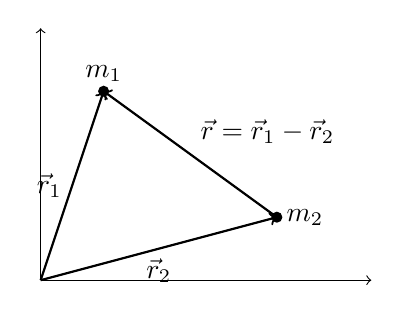
\begin{tikzpicture}[scale=1]
\draw[->] (0,0) -- (4.2,0);
\draw[->] (0,0) -- (0,3.2);
\coordinate (O) at (0,0);
\coordinate (m1) at (0.8,2.4);
\coordinate (m2) at (3.0,0.8);
\draw[thick,->] (O) -- (m1) node[midway,left]{$\vec r_1$};
\draw[thick,->] (O) -- (m2) node[midway,below]{$\vec r_2$};
\draw[thick,->] (m2) -- (m1) node[midway,above right]{$\vec r=\vec r_1-\vec r_2$};
\fill (m1) circle (2pt) node[above]{$m_1$};
\fill (m2) circle (2pt) node[right]{$m_2$};
\end{tikzpicture}
\end{center}

where $\op H$ is given by
\[
\op H=-\frac{\hbar^2}{2m_1}\vec\nabla_1^2-\frac{\hbar^2}{2m_2}\vec\nabla_2^2
+\op V(\vec r_1,\vec r_2,\vec s^{(1)},\vec s^{(2)},\vec t^{(1)},\vec t^{(2)}), 
\]
where $\vec r_i, -i \hbar\vec \nabla_i,  \vec s^{(i)}, \vec t^{(i)}$ (for $i=1,2$) are position, momentum, spin, and isospin operators of first and second nucleon, respectively \footnote{In priciple, nuclenon-nucleon potential can depend also on momenta, but for simplicity we will assume local potential here}. 

A two-body problem can be reduced to an one-body problem if we introduce relative and center-of-mass coordinates
\[
\vec r=\vec r_1-\vec r_2, \qquad
\vec R=\frac{m_1\vec r_1+m_2\vec r_2}{m_1+m_2},
\]
so that
\[
\op H=-\frac{\hbar^2}{2M}\vec\nabla_R^2-\frac{\hbar^2}{2\mu}\vec\nabla_r^2
+\op V(\vec r,\vec R,\vec s^{(1)},\vec s^{(2)},\vec t^{(1)},\vec t^{(2)}),
\qquad M=m_1+m_2,\qquad \mu=\frac{m_1 m_2}{m_1+m_2}.
\]
Further, imposing of translational and rotational invariance, leads to simpler form of $\vec V$, i.e.\ the potential cannot depend on $\vec R$ ,and can depend on $r$ only
$V( r = |\vec r_1-\vec r_2|,\vec s^{(1)},\vec s^{(2)},\vec t^{(1)},\vec t^{(2)})$.

This allows for the factorisation of the wave function
\[
\Psi=\phi_{\rm cm}(\vec R)\,\varphi(\vec r,\vec s^{(1)},\vec s^{(2)},\vec t^{(1)},\vec t^{(2)})
\]
with $\phi_{\rm cm}$ a plane wave describing the center-of-mass (CM) motion,
\[
\phi_{\rm cm}\sim e^{i\vec P\cdot\vec R/\hbar},\qquad
E_{\rm cm}=\frac{P^2}{2M}.
\]
and $\phi$ intrinsic states of the system.

The intrinsic wave function $\phi$ describing  the deuteron (bound) state with the energy $E_d$ must obey Schr\"odinger equation
\begin{equation}
\nonumber
\Big[-\frac{\hbar^2}{2\mu}\vec\nabla_r^2+
\op V( r ,\vec s^{(1)},\vec s^{(2)},\vec t^{(1)},\vec t^{(2)})
\Big]
\varphi(\vec r,\vec s^{(1)},\vec s^{(2)},\vec t^{(1)},\vec t^{(2)})
=E_d\,\varphi(\vec r,\vec s^{(1)},\vec s^{(2)},\vec t^{(1)},\vec t^{(2)}).
\end{equation}
We can express the solution in spherical coordinates
\[
\varphi=R(r)\,Y(\theta,\varphi)\ . \underbrace{\chi_S}_{\text{spin part}} . \underbrace{\chi_T}_{\text{isospin part}}
\]
Let us discuss first spatial part of the wave function. For the moment we can assume, that potential does not depend on spin and isospin (we will see, that one split the problem and solve Schr\"odinger equation for each spin (isospin) channel independently). 

For a potential dependent on $r$, spatial part of wave function can be written as product of radial part $R(r)$ and angular part $Y(\theta, \phi)$. Angular part fulfills
\[
\op L^2 Y=\lambda Y \;\to\; \op L^2 Y_{LM}(\theta,\varphi)=\hbar^2 L(L+1)Y_{LM}(\theta,\varphi),
\qquad L=0,1,2,\dots,\quad M=-L,\dots,L
\]
and represents eigenstates of orbital angular momentum with quantum numbers $L,M$. 

The radial equation
\[
-\frac{\hbar^2}{2\mu}\frac1r\frac{\partial^2}{\partial r^2}(rR)
+\Big[\frac{\hbar^2 L(L+1)}{2\mu r^2}+V\Big]R=E_d R .
\]
can be simplified with the substitution $R(r)=u(r)/r$
\[
R''=\Big(\frac{u'}{r}-\frac{u}{r^2}\Big)'
=\frac{u''}{r}-\frac{u'}{r^2}-\frac{u'}{r^2}+\frac{2u}{r^3},
\qquad
2R'+rR''=u'',
\]
one obtains
\[
-\frac{\hbar^2}{2\mu}u''+\Big[\frac{\hbar^2 L(L+1)}{2\mu r^2}+V\Big]u=E_d\,u .
\]
For given $L$, we will denote solution $u_L(r)$. Let's discuss most simple case, i.e. $L=0$.
\[
-\frac{\hbar^2}{2\mu}u_0''+ V \,u_0=E_d\,u_0,
\]
with boundary condition $u(0)=0$ for a bound state. We can guess that for a short-range potential, the asymptotic ($r\to\infty$) solutions of
$-\frac{\hbar^2}{2\mu}u''=Eu$ are
\[
u(r)\sim e^{\pm ikr}, \qquad k=\frac{\sqrt{2\mu E}}{\hbar}.
\]
Let us refresh the most simple, but still physically meaningful model, the square well-potential 
\begin{center}
\begin{tikzpicture}[scale=1]
\draw[->] (-0.3,1.3) -- (4.5,1.3) node[right]{$r$};
\draw[->] (0,-1.5) -- (0,1.8);
\draw[thick] (0,1.3) -- (0,-1) -- (1.6,-1) -- (1.6,1.3);
\draw[dashed] (0,-1) -- (-0.2,-1) node[left]{$-V_0$};
\draw[dashed] (1.6,1.3) -- (1.6,-1.6) node[below]{$R$};
\end{tikzpicture}
\end{center}

\begin{figure}
    \centering
    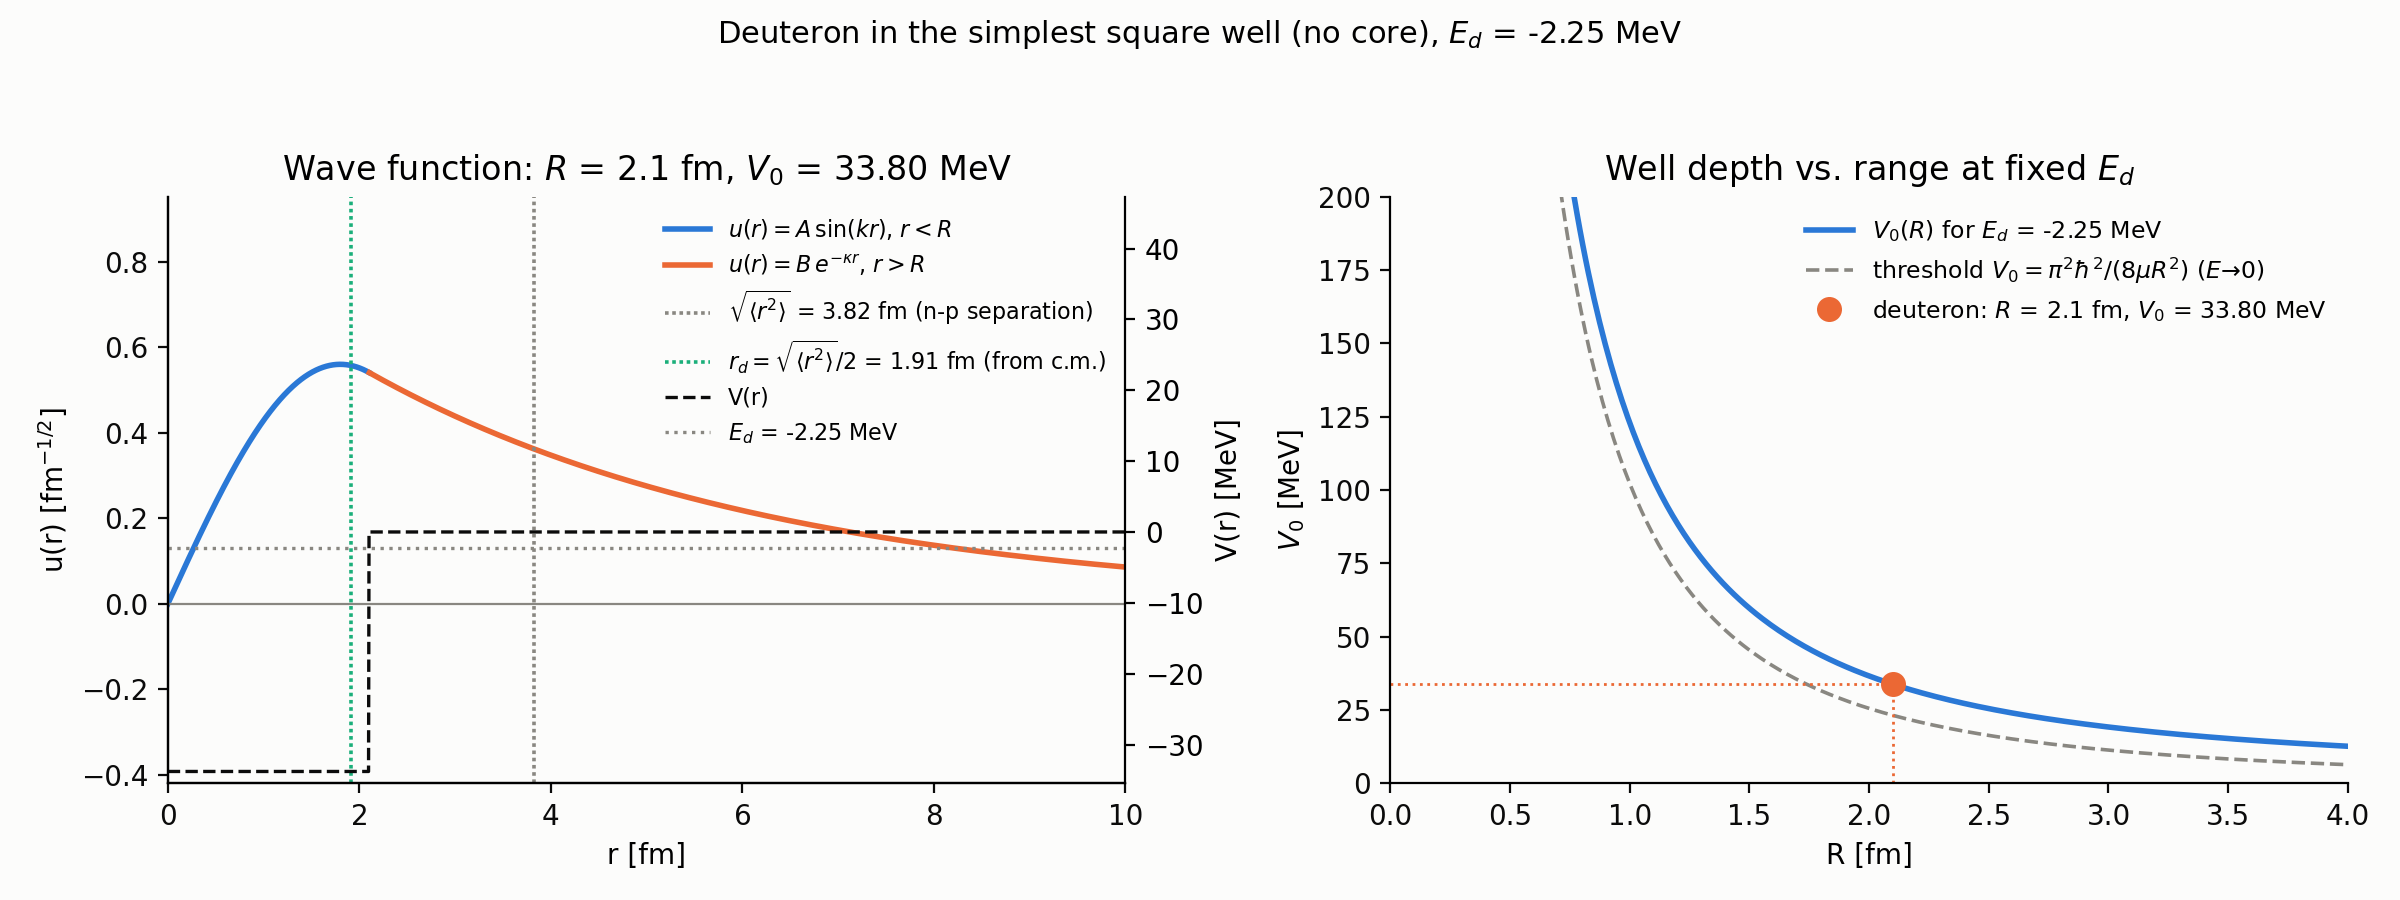
\includegraphics[width=1.0\linewidth]{deuteron_square_well_simple.png}
    \caption{Deuteron wave function in simple square-well model (left). Dependence of well depth  $V_0$ on the width of the well $R$ calculated for deuteron energy $-2.25 MeV$ (right). }
    \label{deuteron_square_well}
\end{figure}

\[
V(r)=
\begin{cases}
-V_0, & r\le R\\
0, & r> R
\end{cases}, \qquad V_0>0 .
\]

\textbf{(1) $r\le R$}
\[
-\frac{\hbar^2}{2\mu}u_0''-(V_0+E_d)u_0=0
\quad\Rightarrow\quad
u_0=A\sin(kr)\ \big[\,\pm B\cos(kr)\ \text{excluded, does not fulfil } u(0)=0\,\big],
\]
\[
k=\frac{\sqrt{2\mu(E_d+V_0)}}{\hbar}.
\]

\textbf{(2) $r\ge R$:}
\[
-\frac{\hbar^2}{2\mu}u_0''-E_d\,u_0=0, \qquad \text{for a bound state } E_d<0,
\]
\[
u\sim e^{\pm\alpha r},\qquad \alpha^2=-\frac{2\mu}{\hbar^2}E_d>0,\qquad
\alpha=\frac{\sqrt{2\mu|E_d|}}{\hbar},
\]
\[
u=B\,e^{-\alpha r}\qquad(e^{\alpha r}\to\infty \text{ as } r\to\infty \text{ is excluded}).
\]

Matching condition at $r=R$:
\[
\left.\frac{u'}{u}\right|_{r=R}:\qquad
\frac{kA\cos(kR)}{A\sin(kR)}=\frac{-\alpha B e^{-\alpha R}}{B e^{-\alpha R}}
\quad\Longrightarrow\quad
\boxed{k\cot(kR)=-\alpha},
\]
\[
\alpha=\frac{1}{\hbar}\sqrt{2\mu|E_d|},\qquad
k=\frac{1}{\hbar}\sqrt{2\mu(E_d+V_0)},\qquad
\mu\approx\frac{m_n}{2}.
\]

For $E_d=-2.25$~MeV (experimental value), solving the matching condition
numerically gives, e.g., $V_0\approx 33.8$~MeV for $R\approx 2.1$~fm (see Fig. \ref{deuteron_square_well}). 


Obviously, radial dependence of the potential influences the shape of the wave function, but in the regime of weakly-bound state and short-range force (like in the case of deuteron) one can obtain qualitatively similar solutions for various shapes of potentials
(see Fig. \ref{deueron_model_comparison}).

Just from experimentally known energy and radius of deuteron we can deduce how the tail of the wave function should look like (where the potential is negligible), but to determine precisely radial dependence of the potential we need to use experimental data from $pn$ scattering (will be discussed later). 

\begin{figure}
    \centering
    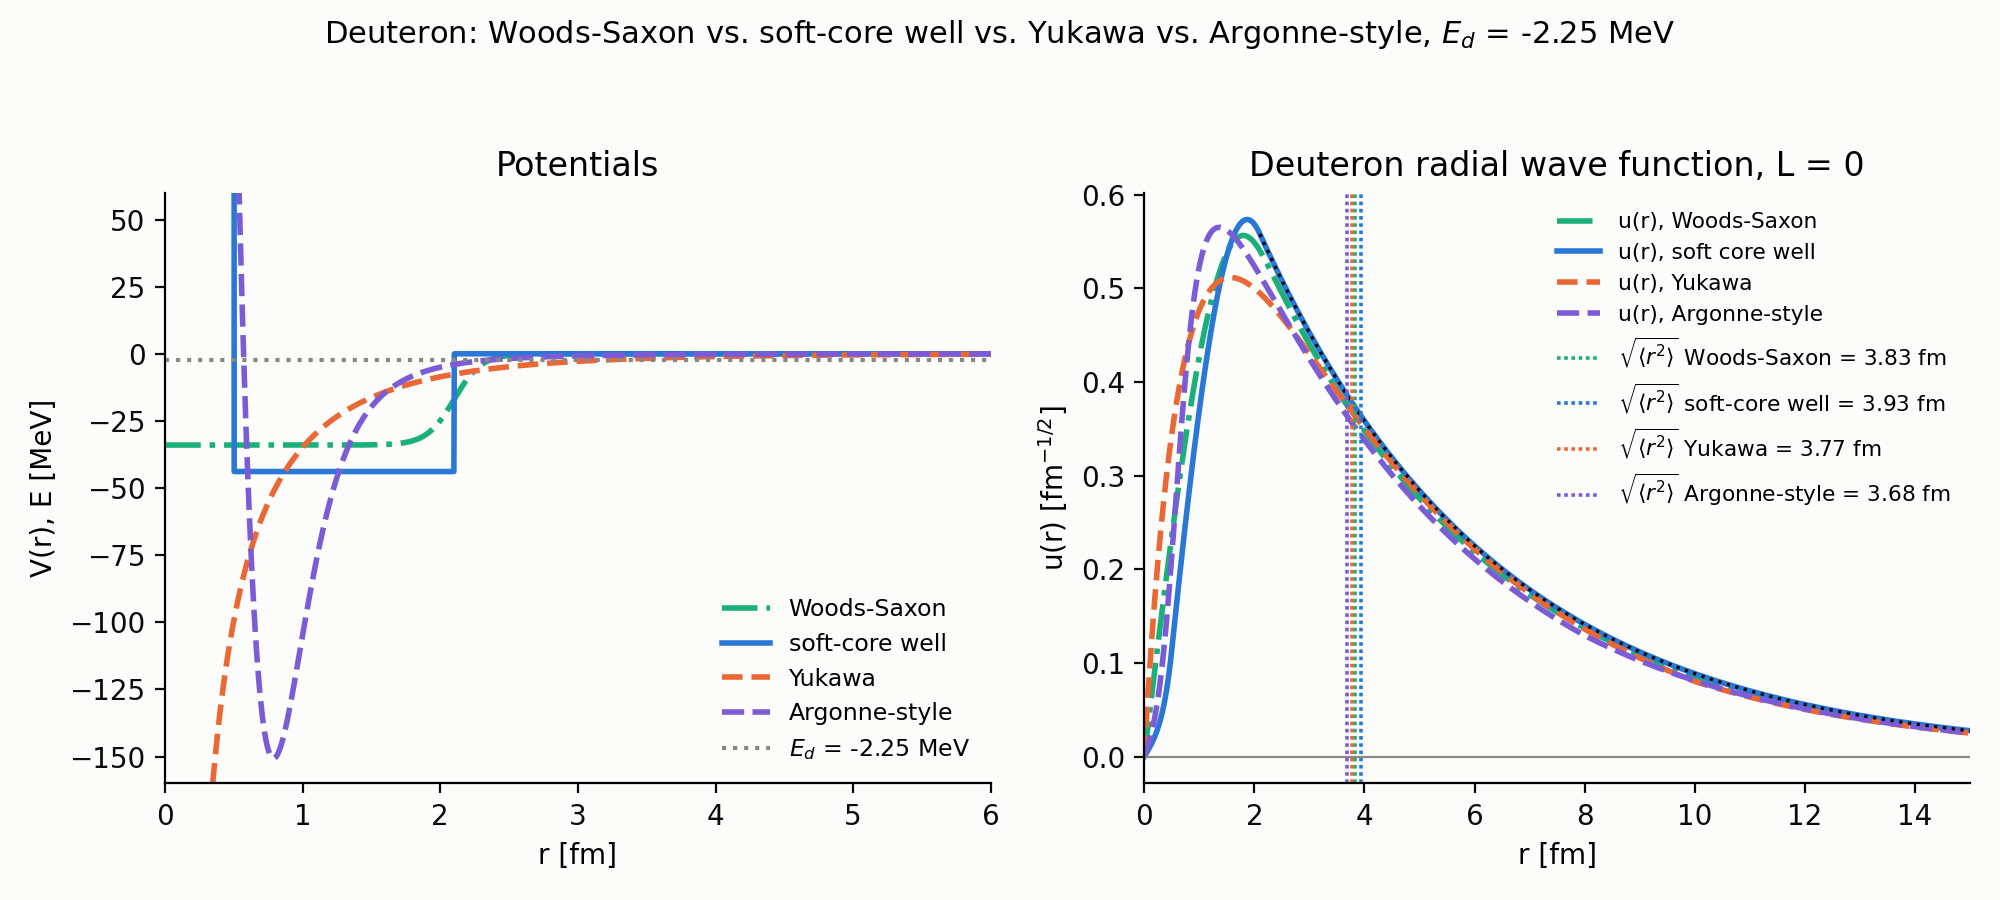
\includegraphics[width=1.0\linewidth]{deuteron_model_comparison.png}
    \caption{Deuteron L=0 wave function calculated for various radial dependencies. Parameters of all potentials are set to reproduce experimental value of deuteron energy $-2.25 MeV$.}
    \label{deueron_model_comparison}
\end{figure}

\subsection{Spin}

The deuteron is the only bound $NN$ state. If we assume isospin invariance of nucleon-nucleon force, the non-existence of other bound (or "almost bound,i.e resonant-like") $NN$ states suggests that it should be $T=0$ state.
Let us assume now, the spin of the deuteron. With intrinsic spins $\vec s^{(1)}$,
$\vec s^{(2)}$ of proton (1) and neutron (2) , the total spin is
\[
\vec S=\vec s^{(1)}+\vec s^{(2)},\qquad S=\tfrac12+\tfrac12=0,1 .
\]
So far we have assumed that orbital momentum is $L=0$, but, in principle, one can also assume $L\ne0$, with a corresponding solution of Schr\"odinger equation for radial function $u_L(r)$. Total spin is then given by $\vec J=\vec L+\vec S$.

Bellow in the table we list possible 2-nucleon states clasified according to $S$ and $T$
We introduce spectroscopic notation 
\[
\qquad {}^{2S+1}L_J, \qquad L=S,P,D,F,\dots \;(0,1,2,3,\dots).
\]

For $L\le 3$ we have the following states:

\begin{center}
\renewcommand{\arraystretch}{1.3}
\begin{tabular}{c c c c c c c}
\hline
$S$ & $L$ & $J^\pi$ & \multicolumn{2}{c}{symmetry of w.f.} & ${}^{2S+1}L_J$ & $T$ \\
 & & & space $(-1)^L$ & spin & & \\
\hline
1 & 0 & $1^+$ & $+$ & $+$ & $\mathbf{{}^3S_1}$ & 0 \\
1 & 2 & $1^+,2^+,3^+$ & $+$ & $+$ & $\mathbf{{}^3D_1},{}^3D_2,{}^3D_3$ & 0 \\
0 & 1 & $1^-$ & $-$ & $-$ & ${}^1P_1$ & 0 \\
0 & 3 & $3^-$ & $-$ & $-$ & ${}^1F_3$ & 0 \\
\hline
1 & 1 & $0^-,1^-,2^-$ & $-$ & $+$ & ${}^3P_0,{}^3P_1,{}^3P_2$ & 1 \\
1 & 3 & $2^-,3^-,4^-$ & $-$ & $+$ & ${}^3F_2,{}^3F_3,{}^3F_4$ & 1 \\
0 & 0 & $0^+$ & $+$ & $-$ & ${}^1S_0$ & 1 \\
0 & 2 & $2^+$ & $+$ & $-$ & ${}^1D_2$ & 1 \\
\hline
\end{tabular}
\end{center}
Let's remind that the $T=0$ can be only $pn$ (antisymmetric in isospin part); whereas the $T=1$ block includes $pn$, $pp$ and $nn$ states (symmetric in isospin part).
Because we know from experiment, that $J^\pi=1^+$ for the deuteron, the state must be either ${}^3S_1$ or ${}^3D_1$.

For a potential that depends only on $r$ with no spin preference, for the $L=0$ state one expects a ${}^1S_0$ bound state, i.e. $J^\pi=0^+$, as well. Since this is \emph{not} the case, we assume that the $NN$
force is \textbf{spin dependent}, i.e. it allows existence of bound state with spin $1^+ (L=0, S=1)$ only. Here we assume, that higher values of $L$ would not allow existence of bound states due to presence of the centrifugal potential for $L>0$. It turns out that situation is more complicated and deuteron is actutally combination of ${}^3S_1$ and ${}^3D_1$ configurations. 

One can introduce simple interaction model mimicking this observation
Let's assume potential of the form 
\[
V=V_0(r)+V_1(r) \op {\vec \sigma}^{(1)} \cdot \op {\vec \sigma}^{(2)}\
\]
where $\op {\vec \sigma}^{\,(i)}, (i=1,2) $ are spin Pauli matrices acting on spin space of first(second) nucleon. 
We can rewrite it in terms of spin operators
\[
\op {\vec S}=\op {\vec s}^{\,(1)}+\op {\vec s}^{\,(2)},
\qquad
\op {\vec s}^{\,(1)}=\tfrac12\op{\vec\sigma}^{(1)},\quad \op {\vec s}^{\,(2)}=\tfrac12\op{\vec\sigma}^{(2)}
\ \ 
\]
\[
\qquad
\op {\vec S}^2=\op {\vec s}^{\,(1)2}+\op {\vec s}^{\,(2)2}+2\,\op {\vec s}^{\,(1)}\!\cdot \op {\vec s}^{\,(2)}
\ \Rightarrow\
V=V_0(r)+2 V_1(r) ( \op {\vec S}^2- \op {\vec s} ^{\,(1)2}-\op {\vec s}^{\,(2)2}).
\]
The solution for such potential can be written as 
\[
\psi_{LS}=R_L(r)\,Y_{Lm_L}(\theta,\varphi)\,\chi^S_{M_S},
\]
where spin part is
\[
\chi^{S=0}_{M_S=0}=\frac{1}{\sqrt2}\Big(\big|\tfrac12\tfrac12\big\rangle^{(1)}\big|\tfrac12{-}\tfrac12\big\rangle^{(2)}
-\big|\tfrac12{-}\tfrac12\big\rangle^{(1)}\big|\tfrac12\tfrac12\big\rangle^{(2)}\Big),
\]
\[
\chi^{S=1}_{M_S=1}=\big|\tfrac12\tfrac12\big\rangle^{(1)}\big|\tfrac12\tfrac12\big\rangle^{(2)},\qquad
\chi^{S=1}_{M_S=-1}=\big|\tfrac12{-}\tfrac12\big\rangle^{(1)}\big|\tfrac12{-}\tfrac12\big\rangle^{(2)},
\]
\[
\chi^{S=1}_{M_S=0}=\frac{1}{\sqrt2}\Big(\big|\tfrac12\tfrac12\big\rangle^{(1)}\big|\tfrac12{-}\tfrac12\big\rangle^{(2)}
+\big|\tfrac12{-}\tfrac12\big\rangle^{(1)}\big|\tfrac12\tfrac12\big\rangle^{(2)}\Big).
\]

The Schr\"odinger equation
\[
\Big[-\frac{\hbar^2}{2\mu}\vec\nabla_r^2+V_0(r)+2V_1(r)\big( \op {\vec S}^2- \op {\vec s} ^{\,(1)2}- \op {\vec s}^{\,(2)2}\big)\Big]\psi_{LS}
=E_{LS}\,\psi_{LS}
\]
can be solved for $S=0,1$ channels separately, i.e. 
\[
S=0:\quad
\Big[-\frac{\hbar^2}{2\mu}\vec\nabla_r^2+V_0+2 V_1 \Big(-\tfrac12\big(\tfrac12{+}1\big)-\tfrac12\big(\tfrac12{+}1\big)\Big)\Big]\psi_{L0}=E_{L0}\psi_{L0},
\qquad
V_{\rm eff}^{S=0}=V_0-3V_1,
\]
\[
S=1:\quad
\Big[-\frac{\hbar^2}{2\mu}\vec\nabla_r^2+V_0+2 V_1\Big(1(1{+}1)-\tfrac12\big(\tfrac12{+}1\big)-\tfrac12\big(\tfrac12{+}1\big)\Big)\Big]\psi_{L1}=E_{L1}\psi_{L1},
\qquad
V_{\rm eff}^{S=1}=V_0+V_1 .
\]
If we assume that $V_0,V_1$ are both attractive in some region,  we can construct a potential which is deep enough for $S=1$ to support a (weakly) bound state, whereas $S=0$ is shallower, with no bound state.

However, as we will see, situation is more complicated, because states with $L>0$ also contribute to the deuteron wave function. In particular this can be directly seen from experimentaly determined values of magnetic dipole and electric quadrupole moments. The fact that $Q>0$ means non-spherical charge distribution and, therefore, the state cannot be pure $S$-wave ($L=0\Rightarrow Y_{00}=1/\sqrt{4\pi}$).

\subsection{\texorpdfstring{${}^3S_1$}{3S1}--\texorpdfstring{${}^3D_1$}{3D1} mixing, magnetic dipole moment and electric quadrupole moment}
Let's assume that deuteron is a linear combination of ${}^3S_1$ and ${}^3D_1$ configurations, i.e.
\[
\psi_{JMS}=\frac{u_0(r)}{r}\big[Y_0\times\chi^{S=1}\big]^{J=1}_M
+\frac{u_2(r)}{r}\big[Y_2\times\chi^{S=1}\big]^{J=1}_M,
\]
where
\[
\big[Y_L\times\chi^S\big]^J_M=\sum_{m_L,m_S}\big(Lm_L\,Sm_S\,|\,JM\big)\,Y_{Lm_L}(\theta,\varphi)\,\chi^S_{m_S}.
\]
Radial parts of wave function $u_0,u_2$ fulfill radial Schr\"odinger equation for $L=0,2$. Let us evaluate magnetic dipole moment for such state. We evaluate magnetic dipole moment as expectation value of $z-$ component of magnetic dipole operator in the state with maximal value of angular momentum projection (this is usuall convention), i. e for $J=1,\ M=1,\ S=1$. The wave function is explicitly given by 
\[
\psi_{111}=\frac{u_0}{r}\sum_{m_L,m_S}Y_{0m_L}\chi^1_{m_S}(0m_L\,1m_S|11)
+\frac{u_2}{r}\sum_{m_L,m_S}Y_{2m_L}\chi^1_{m_S}(2m_L\,1m_S|11)
\]
\[
=\frac{u_0}{r}Y_{00} \chi^1_1
+\frac{u_2}{r}\Big[\sqrt{\tfrac35}\,Y_{22}\chi^1_{-1}-\sqrt{\tfrac{3}{10}}\,Y_{21}\chi^1_0
+\sqrt{\tfrac{1}{10}}\,Y_{20}\chi^1_1\Big].
\]
(relevant Clebsh-Gordan coefficients are $(221-1|11)=\sqrt{\frac{3}{5}}, (2110|11)=-\sqrt{\frac{3}{10}}, (2011|11)=\sqrt{\frac{1}{10}}$.)

Magnetic dipole moment is given by
\[
\mu=\braket{\psi_{111}|\op\mu_z|\psi_{111}},
\qquad
\op\mu_z=g_s^p\,\op s_z^p+g_s^n\,\op s_z^n+g_\ell^p\,\op\ell_z^p
\quad(\text{in units of }\mu_N=\frac{e \hbar}{2m_p}),
\]
\[
g_s^p=5.5855,\qquad g_\ell^p=1,\qquad g_s^n=-3.8263,
\]
where $g_s^p,g_s^n,g_l^p$, are corresponding proton and neutron spin and orbital gyromagnetic factors. 

Lets' express $\op \mu_z$ by using relative coordinates. We have
$\vec R=\tfrac12( \vec {r^p}+\vec {r^n})$, $m_p\approx m_n\approx m$,
$\vec r=\vec {r^p}-\vec {r^n}$, therefore, $\vec {r^p}=\vec R+\tfrac{\vec r}{2}$, $\vec
{r^n}=\vec R-\tfrac{\vec r}{2}$, and $ \vec P=\vec {p^p}+\vec {p^n}$,
$\vec p=\tfrac12(\vec {p^p}-\vec {p^n})$, or ,  $\vec {p^p}=\tfrac{\vec P}{2}+\vec p$,
$\vec {p^n}=\tfrac{\vec P}{2}-\vec p$. Then
\[
\vec\ell^p=\vec {r^p}\times\vec {p^p}=(\vec R +\tfrac{\vec r}{2})\times(\frac{\vec P}{2}+ \vec p) 
\]
Since we are not interested in translational part given by $\vec P$, and in CM frame $\vec R = 0$, we can write for orbital angular momentum 
\[
\vec\ell^p=\frac{\vec L}{2},\qquad\text{where} \qquad \vec L = \vec r \times \vec p.   
\]
Therefore, the operator of dipole moment ($z$-component) can be writtes as 

\[
\op\mu_z=g_s^p\op s_z^p+g_s^n\op s_z^n+\tfrac12\op L_z
\]

Using the orthonormality relations
\[
\chi^{S\dagger}_{m_S}\chi^{S'}_{m_S'}=\delta_{SS'}\delta_{m_Sm_S'},\qquad
\int \ud\Omega\, Y^*_{Lm_L}(\Omega)\,Y_{L'm_L'}(\Omega)=\delta_{LL'}\delta_{m_Lm_L'},
\]
\[
(\text{we use shorthand notation   }
\Omega = (\theta, \phi), 
\int \ud \Omega  = \int_0^{2\pi}\!\ud\varphi\int_0^\pi\!\sin\theta\,\ud\theta\ )
\]
we obtain for magnetic moment
\[
\mu=\braket{\psi_{111}|\op\mu_z|\psi_{111}}=\int_0^\infty \ud r\, u_0^2\,
\Big(g_s^p\,\chi^{1\dagger}_1\op s_z^p\chi^1_1+g_s^n\,\chi^{1\dagger}_1\op s_z^n\chi^1_1
+\tfrac12\!\!\underbrace{\int\ud\Omega\,Y^*_{00}\op L_zY_{00}}_{0}\!\!\Big)
\]
\[
+\int_0^\infty \ud r\, u_2^2\,\Big\{
\tfrac35\Big(g_s^p\chi^{1\dagger}_{-1}\op s_z^p\chi^1_{-1}+g_s^n\chi^{1\dagger}_{-1}\op s_z^n\chi^1_{-1}
+\tfrac12\!\!\underbrace{\int\ud\Omega\,Y^*_{22}\op L_zY_{22}}_{=2}\!\!\Big)
\]
\[
+\tfrac{3}{10}\Big(g_s^p\chi^{1\dagger}_0\op s_z^p\chi^1_0+g_s^n\chi^{1\dagger}_0\op s_z^n\chi^1_0
+\tfrac12\!\!\underbrace{\int\ud\Omega\,Y^*_{21}\op L_zY_{21}}_{=1}\!\!\Big)
+\tfrac{1}{10}\Big(g_s^p\chi^{1\dagger}_1\op s_z^p\chi^1_1+g_s^n\chi^{1\dagger}_1\op s_z^n\chi^1_1
+\tfrac12\!\!\underbrace{\int\ud\Omega\,Y^*_{20}\op L_zY_{20}}_{= 0}\!\!\Big)\Big\},
\]
with
\[
\chi^1_1=\big|\tfrac12\tfrac12\big\rangle^p\big|\tfrac12\tfrac12\big\rangle^n, \quad
\chi^{1\dagger}_1\op s_z^p\chi^1_1=\chi^{1\dagger}_1\op s_z^n\chi^1_1=\tfrac12
\qquad
\chi^1_{-1}=\big|\tfrac12{-}\tfrac12\big\rangle^p\big|\tfrac12{-}\tfrac12\big\rangle^n,\quad
\chi^{1\dagger}_{-1}\op s_z^p\chi^1_{-1}=\chi^{1\dagger}_{-1}\op s_z^n\chi^1_{-1}=-\tfrac12,
\]
\[
\chi^1_0=\tfrac{1}{\sqrt2}\Big(\big|\tfrac12\tfrac12\big\rangle^p\big|\tfrac12{-}\tfrac12\big\rangle^n
+\big|\tfrac12{-}\tfrac12\big\rangle^p\big|\tfrac12\tfrac12\big\rangle^n\Big),\qquad
\chi^{1\dagger}_0\op s_z^p\chi^1_0=\chi^{1\dagger}_0\op s_z^n\chi^1_0=0 .
\]
Therefore
\[
\mu=\tfrac12\big(g_s^n+g_s^p\big)\int_0^\infty u_0^2\,\ud r
+\int_0^\infty u_2^2\,\ud r\,
\Big\{\tfrac35\Big[-\tfrac12(g_s^p+g_s^n)+1\Big]+\tfrac{3}{10}\cdot\tfrac12+\tfrac{1}{10}\cdot\tfrac12(g_S^n+g_S^p)\Big\}
\]
\[
=\tfrac12(g_s^p+g_s^n)\int_0^\infty u_0^2\,\ud r
+\Big[\tfrac34-\tfrac14(g_s^p+g_s^n)\Big]\int_0^\infty u_2^2\,\ud r .
\]

With the normalisation $\braket{\psi_{111}|\psi_{111}}=1\Rightarrow
\int_0^\infty(u_0^2+u_2^2)\,\ud r=1$, and defining the $D$-state probability
$w_D\equiv\int_0^\infty u_2^2\,\ud r$,
\[
\mu=\tfrac12(g_s^p+g_s^n)\big(1-w_D\big)+\Big[\tfrac34-\tfrac14(g_s^p+g_s^n)\Big]w_D
=\tfrac12(g_s^p+g_s^n)-\Big[\tfrac34(g_s^p+g_s^n)-\tfrac34\Big]w_D .
\]

Experimentally, $\mu=\mu^p+\mu^n-0.0222=\tfrac12(g_s^p+g_s^n)-0.0222$ , so the
$D$-state probability is
\[
w_D \approx
\frac{0.0222}{\tfrac34(g_s^p+g_s^n)-\tfrac34} \approx  0.039.
\]
From the expertimental value of dipole magnetic moment we therefore estimate probability of $D-$ wave in the deuteron to be $\approx$ 4\%.

Within the same model we can calculate electric quadrupole moment. Electric quadrupole moment is a tensor with components given by
\[
Q_{ij}=\int \ud^3r\,\big(3r_ir_j-\delta_{ij}r^2\big)\,\rho^{\rm ch}(\vec r)
\]
where $\rho^{ch}(\vec r)$ is charged density, which for the deuteron is approximated by  point-like proton density
\[
\qquad
\rho^{\rm ch}(\vec r)\approx\rho^p(\vec r)=\delta(\vec r-\vec r^{\,p}).
\]
It is natural to introduce quadrupole tensor operator
\[
\op Q_{ij}=3\op r^{p}_i\op r^{p}_j - \delta_{ij}{(\op \vec{r^p})}^2
\]
The convention is to define electric quadrupole moment (number) for axially symmetric distribution as
expectation value of $\op Q_{33}$ (expressed  in coordinate system where quadrupole tensor is diagonal) for state with maximal projection, i.e 
\[
\qquad
Q \equiv \bra {\psi_{111}} \op Q_{33} \ket {\psi_{111}}=\bra {\psi_{111}} \Big[3(\hat z^{\,p})^2-{(\op r^{p})}^2\Big] \ket {\psi_{111}}.
\]
In the CM system, $\vec r=\vec r^{\,p}-\vec r^{\,n}\approx 2\vec r^{\,p}$ (since
$m_p\approx m_n\Rightarrow \vec r^{\,p}=-\vec r^{\,n}$), so
\[
\op Q_{33}=\frac{1}{4}\big(3\op z^2-\op r^2\big)=\Big(\frac{\pi}{5}\Big)^{1/2}\op r^2\,\op Y_{20}(\theta,\varphi).
\]
After rather straightforward evaluation one gets for deuteron quadrupole moment
\[
Q =\frac{1}{10}\int_0^\infty\Big(\sqrt{2} u_0 (r) u_2 (r) -\tfrac12 u_2(r)^2\Big)\,r^2\,\ud r .
\]
One can observe, that nonzero value of $Q$ originates from the presense of $u_2$ in the integral, i.e. contribution of the $D-$ wave part of the wave function. Unlike to magnetic dipole moment it depends on radial part of the wave function and is therefore sensitive to radial dependence of potential. 

\subsection {Properties of NN interaction}
We have already argued that the deuteron is a mixture of states with different orbital angular momentum $L$. However, an interaction of the type
\[
V_1(r)+V_2(r)\,f\big(\vec\sigma^{(1)},\vec\sigma^{(2)}\big)
\]
does not mix states with differen $L$, and is essentially a part of central force. Even without details about radial dependence one can deduce basic structure of general potential wchich includes spin and isospin dependence.  
We can use basic symmetries to restrict form of the $NN$ potential are:

\[
V=V\big(\vec r^{(1)},\vec r^{(2)},\vec p^{(1)},\vec p^{(2)},\vec\sigma^{(1)},\vec\sigma^{(2)},
\vec\tau^{(1)},\vec\tau^{(2)}\big)\equiv V(1,2),
\qquad
V(1,2)\stackrel{!}{=}V(2,1).
\]

\textbf{Translational invariance:} $\vec r^{(1)}\to\vec r^{(1)}+\vec a$,
$\vec r^{(2)}\to\vec r^{(2)}+\vec a$, $\forall\vec a$. With
\[
\vec r=\vec r^{(1)}-\vec r^{(2)},\qquad \vec R=\tfrac12(\vec r^{(1)}+\vec r^{(2)}),\qquad
\vec p=\frac{\vec p^{(1)}-\vec p^{(2)}}{2},\qquad \vec P=\vec p^{(1)}+\vec p^{(2)},
\]
\[
V\big(\vec r,\vec R,\vec p,\vec P,\vec\sigma^{(1)},\vec\sigma^{(2)},\vec\tau^{(1)},\vec\tau^{(2)}\big)
\stackrel{!}{=}V\big(\vec r,\vec R+\vec a,\vec p,\vec P,\dots\big)
\quad\Rightarrow\quad V \text{ cannot depend on } \vec R .
\]

\textbf{Invariance with respect to Galilean transformation:}
$\vec p^{(1)}\to\vec p^{(1)}+\vec p_0$, $\vec p^{(2)}\to\vec p^{(2)}+\vec p_0$, $\forall\vec p_0$:
\[
V\big(\vec r,\vec p,\vec P,\vec\sigma^{(1)},\vec\sigma^{(2)},\vec\tau^{(1)},\vec\tau^{(2)}\big)
\stackrel{!}{=}V\big(\vec r,\vec p,\vec P+2\vec p_0,\vec\sigma^{(1)},\vec\sigma^{(2)},\vec\tau^{(1)},\vec\tau^{(2)}\big)
\]
$\Rightarrow$ $V$ cannot depend on $\vec P$:
\[
\op V=\op V\big(\vec r,\vec p,\vec\sigma^{(1)},\vec\sigma^{(2)},\vec\tau^{(1)},\vec\tau^{(2)}\big).
\]

\textbf{Invariance with respect to parity transformation:}
\[
\op V\big(\vec r,\vec p,\vec\sigma^{(1)},\vec\sigma^{(2)},\vec\tau^{(1)},\vec\tau^{(2)}\big)
\stackrel{!}{=}\op V\big(-\vec r,-\vec p,\vec\sigma^{(1)},\vec\sigma^{(2)},\vec\tau^{(1)},\vec\tau^{(2)}\big).
\]

\textbf{Time reversal invariance:}
\[
\op V\big(\vec r,\vec p,\vec\sigma^{(1)},\vec\sigma^{(2)},\vec\tau^{(1)},\vec\tau^{(2)}\big)
\stackrel{!}{=}\op V\big(\vec r,-\vec p,-\vec\sigma^{(1)},-\vec\sigma^{(2)},\vec\tau^{(1)},\vec\tau^{(2)}\big).
\]

\textbf{Rotational invariance:}
will be discussed later.
\newline
\newline
Note about most general dependence on \texorpdfstring{$\vec\sigma^{(1)},\vec\sigma^{(2)}$}{sigma1, sigma2}:

The most general function $f\big(\vec r,\vec p,\vec\sigma^{(1)},\vec\sigma^{(2)}\big)$ can be decomposed to
\[
f\big(\vec r,\vec p,\vec\sigma^{(1)},\vec\sigma^{(2)}\big)
=\sum_{i,j=0}^{3}V_{ij}(\vec r,\vec p)\,\sigma_i^{(1)}\sigma_j^{(2)},
\qquad
\sigma_0^{(\alpha)}=\mathbbm{1} ,\quad \sigma_1^{(\alpha)}=\sigma_x^{(\alpha)},\quad \sigma_2^{(\alpha)}=\sigma_y^{(\alpha)},\quad \sigma_3^{(\alpha)}=\sigma_z^{(\alpha)},
\]
, i.e. spin dependent part can expressed it in terms $\sim\sigma_i^{(1,2)}$, $\ \sigma_i^{(1)}\sigma_j^{(2)}$.
More complicated terms $\sigma_i^{(\alpha)}\sigma_j^{(\alpha)}\sigma_k^{(\alpha)}$
can be reduced to $\sim\sigma_i^{(1,2)}$, $\sigma_i^{(1)}\sigma_j^{(2)}$, since
\[
\left.
\begin{aligned}
\big[\sigma_i^{(\alpha)},\sigma_j^{(\alpha)}\big]&=2i\,\varepsilon_{ijk}\,\sigma_k^{(\alpha)}\\
\big\{\sigma_i^{(\alpha)},\sigma_j^{(\alpha)}\big\}&=2\,\mathbbm{1} \delta_{ij}
\end{aligned}
\right\}
\quad\Rightarrow\quad
\sigma_i^{(\alpha)}\sigma_j^{(\alpha)}=\mathbbm{1} \delta_{ij}+i\,\varepsilon_{ijk}\,\sigma_k^{(\alpha)} .
\]

One can construct different operatorial terms from basic operators $\vec \sigma,\vec r,\vec p$ 

Important symmetries:
$\mathcal P$ --- parity ($\vec r\to-\vec r$), $\mathcal T$ --- time inversion ($t\to-t$).

Spin space:
\begin{center}
\renewcommand{\arraystretch}{1.3}
\begin{tabular}{l c c c}
\hline
\multicolumn{2}{l}{spin space} & $\mathcal P$ & $\mathcal T$ \\
\hline
scalar & $\mathbbm{1}$ & $+$ & $+$ \\
scalar & $\vec\sigma^{(1)}\!\cdot\vec\sigma^{(2)}$ & $+$ & $+$ \\
vector & $\vec\sigma^{(1)}\times\vec\sigma^{(2)}$ & $+$ & $+$ \\
vector & $\vec\sigma^{(1)}-\vec\sigma^{(2)}$ & $+$ & $-$ \\
vector & $\vec\sigma^{(1)}+\vec\sigma^{(2)}$ & $+$ & $-$ \\
tensor & $\big[\sigma^{(1)}\times\sigma^{(2)}\big]^2_m$ & $+$ & $+$ \\
\hline
\end{tabular}
\end{center}
with
\[
\big[\sigma^{(1)}\times\sigma^{(2)}\big]^2_m=\sum_{m_1m_2}\big(1m_1\,1m_2\,|\,2m\big)\,
\sigma^{(1)}_{1m_1}\sigma^{(2)}_{1m_2},
\]
\[
\sigma^{(\alpha)}_{10}=\sigma^{(\alpha)}_z,\quad
\sigma^{(\alpha)}_{1\pm1}=\mp\frac{1}{\sqrt2}\big(\sigma^{(\alpha)}_x\pm i\sigma^{(\alpha)}_y\big),
\quad \alpha=1,2 .
\]

Coordinate space $(\vec r,\vec p)$:
\begin{center}
\renewcommand{\arraystretch}{1.3}
\begin{tabular}{l c c c}
\hline
 & & $\mathcal P$ & $\mathcal T$ \\
\hline
scalar & $\vec r^{\,2}$ & $+$ & $+$ \\
scalar & $\vec p^{\,2}$ & $+$ & $+$ \\
scalar & $\vec r\cdot\vec p$ & $+$ & $-$ \\
vector & $\vec r$ & $-$ & $+$ \\
vector & $\vec p$ & $-$ & $-$ \\
vector & $\vec r\times\vec p$ & $+$ & $-$ \\
tensor & $\big[r_1\times p_1\big]^2_m$ & $+$ & $-$ \\
tensor & $\big[r_1\times r_1\big]^2_m$ & $+$ & $+$ \\
tensor & $\big[p_1\times p_1\big]^2_m$ & $+$ & $+$ \\
\hline
\end{tabular}
\end{center}
where $r_1$, $p_1$ denote the rank-1 (spherical) tensors built from $\vec r$, $\vec p$:
\[
\big[r_1\times r_1\big]^2_m=\sum_{m_1m_2}\big(1m_1\,1m_2\,|\,2m\big)\,r_{1m_1}r_{1m_2},
\qquad
r_{10}=z,\qquad r_{1\pm1}=\mp\frac{1}{\sqrt2}(x\pm iy).
\]

The Hamiltonian can contain only scalars. We search for vector--vector and
tensor--tensor products invariant under $\mathcal P$ and $\mathcal T$:

\textbf{Vector--vector:}
\[
(\vec r\times\vec p)\cdot\big(\vec\sigma^{(1)}+\vec\sigma^{(2)}\big)=2\,\vec L\cdot\vec S ,
\]
$(\vec r\times\vec p)\cdot\big(\vec\sigma^{(1)}-\vec\sigma^{(2)}\big)$ is not considered, because it is not  invariant under the $1\leftrightarrow2$ exchange.

\textbf{Tensor--tensor:}
\begin{center}
\renewcommand{\arraystretch}{1.3}
\begin{tabular}{l c c c c}
\hline
 & \multicolumn{2}{c}{spin part} & \multicolumn{2}{c}{space part}\\
 & $\mathcal P$ & $\mathcal T$ & $\mathcal P$ & $\mathcal T$ \\
\hline
$\big[r_1\times r_1\big]^2\cdot\big[\sigma^{(1)}_1\times\sigma^{(2)}_1\big]^2$ & $+$ & $+$ & $+$ & $+$ \\
$\big[p_1\times p_1\big]^2\cdot\big[\sigma^{(1)}_1\times\sigma^{(2)}_1\big]^2$ & $+$ & $+$ & $+$ & $+$ \\
$\big[\sigma^{(1)}\times\sigma^{(2)}\big]^2\cdot\big[r_1\times p_1\big]^2\,(\vec r\cdot\vec p)$ & $+$ & $+$ & $+$\,$\cdot$\,$+$ & $-$\,$\cdot$\,$-$ \\
\hline
\end{tabular}
\end{center}
Let's remind definition of tensor scalar product:
\[
A^\lambda\cdot B^\lambda=(-1)^\lambda\sqrt{2\lambda+1}\,\big[A^\lambda\times B^\lambda\big]^0_0,
\qquad
\text{so e.g.}
\big[r_1\times r_1\big]^2\cdot\big[\sigma^{(1)}_1\times\sigma^{(2)}_1\big]^2
=\sqrt5\,\Big[\big[r_1\times r_1\big]^2\times\big[\sigma^{(1)}\times\sigma^{(2)}\big]^2\Big]^0_0 .
\]
One can easily show relation
\[
\big[r_1\times r_1\big]^2\cdot\big[\sigma^{(1)}_1\times\sigma^{(2)}_1\big]^2
=\big(\vec\sigma^{(1)}\!\cdot\vec r\big)\big(\vec\sigma^{(2)}\!\cdot\vec r\big)
-\tfrac13\,\vec\sigma^{(1)}\!\cdot\vec\sigma^{(2)}\,r^2 .
\]
It is common to define the "tensor interaction" term
\[
\op V\equiv V_T\,\op S_{12},
\qquad
\op S_{12}=\frac{3}{r^2}\big(\vec\sigma^{(1)}\!\cdot\vec r\big)\big(\vec\sigma^{(2)}\!\cdot\vec r\big)
-\vec\sigma^{(1)}\!\cdot\vec\sigma^{(2)}
=3\big(\vec\sigma^{(1)}\!\cdot\vec n_r\big)\big(\vec\sigma^{(2)}\!\cdot\vec n_r\big)
-\vec\sigma^{(1)}\!\cdot\vec\sigma^{(2)} .
\]

\subsubsection*{Classical picture}

\begin{center}
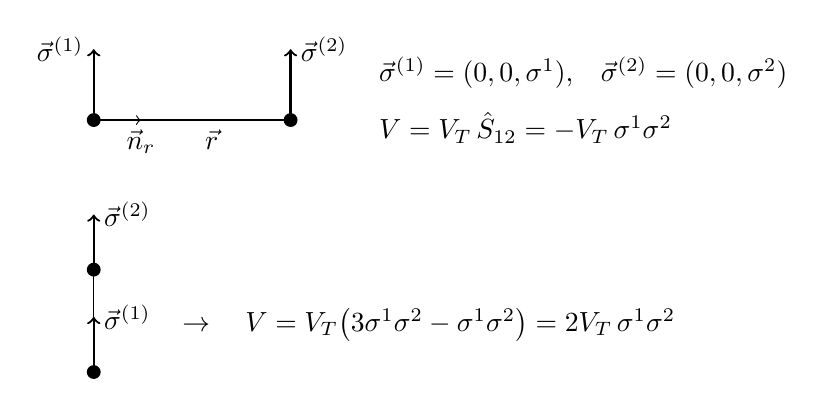
\begin{tikzpicture}[scale=1]
% spins perpendicular to r
\fill (0,0) circle (2.5pt);
\fill (2.5,0) circle (2.5pt);
\draw (0,0) -- (2.5,0);
\draw[thick,->] (0,0) -- (0,0.9) node[left]{$\vec\sigma^{(1)}$};
\draw[thick,->] (2.5,0) -- (2.5,0.9) node[right]{$\vec\sigma^{(2)}$};
\draw[->] (0,0) -- (0.6,0) node[below]{$\vec n_r$};
\node[below] at (1.5,0) {$\vec r$};
\node[right] at (3.5,0.6) {$\vec\sigma^{(1)}=(0,0,\sigma^1)$,\quad $\vec\sigma^{(2)}=(0,0,\sigma^2)$};
\node[right] at (3.5,-0.1) {$V=V_T\,\op S_{12}=-V_T\,\sigma^1\sigma^2$};
% spins parallel to r
\begin{scope}[yshift=-3.2cm]
\fill (0,0) circle (2.5pt);
\fill (0,1.3) circle (2.5pt);
\draw (0,0) -- (0,1.3);
\draw[thick,->] (0,0) -- (0,0.7) node[right]{$\vec\sigma^{(1)}$};
\draw[thick,->] (0,1.3) -- (0,2.0) node[right]{$\vec\sigma^{(2)}$};
\node[right] at (1.0,0.6) {$\to\quad V=V_T\big(3\sigma^1\sigma^2-\sigma^1\sigma^2\big)=2V_T\,\sigma^1\sigma^2$};
\end{scope}
\end{tikzpicture}
\end{center}
$\Rightarrow$ the force is not central.

\subsection{Deuteron with tensor interaction}

Tensor interaction $\to$ mixing of states with different $L$. For the deuteron
\[
\op V=\op V_C+V_T\,\op S_{12},
\]
with $\op V_C$ the central and $V_T\op S_{12}$ the tensor part (both can depend
on spins, isospins, \dots).

Wave function:
\[
\psi_{JM}=\sum_L\psi_{LSJM},
\qquad
\psi_{LSJM}=\frac{u_L}{r}\underbrace{\sum_{m_Lm_S}\big(Lm_L\,Sm_S\,|\,JM\big)\,
Y_{Lm_L}(\theta,\varphi)\,\chi^S_{m_S}}_{\displaystyle\bar\varphi_{LSJM}}
\equiv\frac{u_L}{r}\,\bar\varphi_{LSJM} .
\]

Deuteron: $J=1$, $S=1$, $L=0,2$:
\[
\psi^{deut.}_{JM}=\psi_{011M}+\psi_{211M}.
\]

Schr\"odinger equation:
\begin{multline*}
\Big[-\frac{\hbar^2}{2\mu}\Big(\frac{\partial^2}{\partial r^2}+\frac2r\frac{\partial}{\partial r}
-\frac{1}{\hbar^2r^2}\op L^2\Big)+V_C+V_T\op S_{12}\Big]\big(\psi_{011M}+\psi_{211M}\big)\\
=E\big(\psi_{011M}+\psi_{211M}\big)
\qquad\Big/\ \int\!\ud\Omega\,\bar\varphi^\dagger_{011M},\ \ \int\!\ud\Omega\,\bar\varphi^\dagger_{211M}.
\end{multline*}
Projecting onto $\bar\varphi_{011M}$:
\begin{multline*}
\Big[-\frac{\hbar^2}{2\mu}\Big(\frac{\partial^2}{\partial r^2}+\frac2r\frac{\partial}{\partial r}\Big)+V_C\Big]
\frac{u_0}{r}\int\bar\varphi^\dagger_{011M}\bar\varphi_{011M}\,\ud\Omega\\
+\Big[-\frac{\hbar^2}{2\mu}\Big(\frac{\partial^2}{\partial r^2}+\frac2r\frac{\partial}{\partial r}
-\frac{2(2+1)}{r^2}\Big)+V_C\Big]\frac{u_2}{r}
\underbrace{\int\bar\varphi^\dagger_{011M}\bar\varphi_{211M}\,\ud\Omega}_{=\,0}\\
+V_T\frac{u_0}{r}\int\bar\varphi^\dagger_{011M}\op S_{12}\bar\varphi_{011M}\,\ud\Omega
+V_T\frac{u_2}{r}\int\bar\varphi^\dagger_{011M}\op S_{12}\bar\varphi_{211M}\,\ud\Omega\\
=E\Big(\frac{u_0}{r}\int\bar\varphi^\dagger_{011M}\bar\varphi_{011M}\,\ud\Omega
+\frac{u_2}{r}\underbrace{\int\bar\varphi^\dagger_{011M}\bar\varphi_{211M}\,\ud\Omega}_{=\,0}\Big).
\end{multline*}

\emph{Note:}
\begin{multline*}
\int\!\ud\Omega\,\bar\varphi^\dagger_{LSJM}\,\bar\varphi_{L'S'J'M'}\\
=\sum_{\substack{m_Lm_L'\\ m_Sm_S'}}\big(Lm_L\,Sm_S\,|\,JM\big)\big(L'm_L'\,S'm_S'\,|\,J'M'\big)
\underbrace{\int\!\ud\Omega\,Y^*_{Lm_L}(\Omega)\,Y_{L'm_L'}(\Omega)}_{\delta_{LL'}\delta_{m_Lm_L'}}
\underbrace{\chi^{S\dagger}_{m_S}\chi^{S'}_{m_S'}}_{\delta_{SS'}\delta_{m_Sm_S'}}
\end{multline*}
\[
=\delta_{LL'}\delta_{SS'}\sum_{m_Sm_L}\big(Lm_L\,Sm_S\,|\,JM\big)\big(Lm_L\,Sm_S\,|\,J'M'\big)
=\delta_{JJ'}\delta_{MM'}\delta_{LL'}\delta_{SS'} .
\]
\begin{multline*}
\Rightarrow\quad
-\frac{\hbar^2}{2\mu}\Big(\frac{\partial^2}{\partial r^2}+\frac2r\frac{\partial}{\partial r}\Big)\frac{u_0}{r}
+V_C\frac{u_0}{r}+V_T\frac{u_0}{r}\big(011M\big|\op S_{12}\big|011M\big)\\
+V_T\frac{u_2}{r}\big(011M\big|\op S_{12}\big|211M\big)=E\frac{u_0}{r},
\end{multline*}
\[
\boxed{
\begin{aligned}
-\frac{\hbar^2}{2\mu}u_0''+V_C\,u_0
&+V_T\,u_0\big(011M\big|\op S_{12}\big|011M\big)\\
&+V_T\,u_2\big(011M\big|\op S_{12}\big|211M\big)=E\,u_0
\end{aligned}
}
\]
where
\[
\big(LSJM\big|\op S_{12}\big|L'S'J'M'\big)\equiv\int\!\ud\Omega\,\bar\varphi^\dagger_{LSJM}\,\op S_{12}\,\bar\varphi_{L'S'J'M'} .
\]

In analogy,
\begin{multline*}
-\frac{\hbar^2}{2\mu}\Big(\frac{\partial^2}{\partial r^2}+\frac2r\frac{\partial}{\partial r}
-\frac{2(2+1)}{r^2}\Big)\frac{u_2}{r}+V_C\frac{u_2}{r}\\
+V_T\frac{u_0}{r}\big(211M\big|\op S_{12}\big|011M\big)
+V_T\frac{u_2}{r}\big(211M\big|\op S_{12}\big|211M\big)=E\frac{u_2}{r},
\end{multline*}
\[
\boxed{
\begin{aligned}
-\frac{\hbar^2}{2\mu}u_2''+\Big(V_C+\frac{6\hbar^2}{2\mu r^2}\Big)u_2
&+V_T\,u_0\big(211M\big|\op S_{12}\big|011M\big)\\
&+V_T\,u_2\big(211M\big|\op S_{12}\big|211M\big)=E\,u_2
\end{aligned}
}
\]

We got 2 coupled differential equations for the radial wave functions, with the
normalisation condition
\[
\int_0^\infty\big(u_0^2+u_2^2\big)\,\ud r=1 .
\]

\begin{figure}
    \centering
    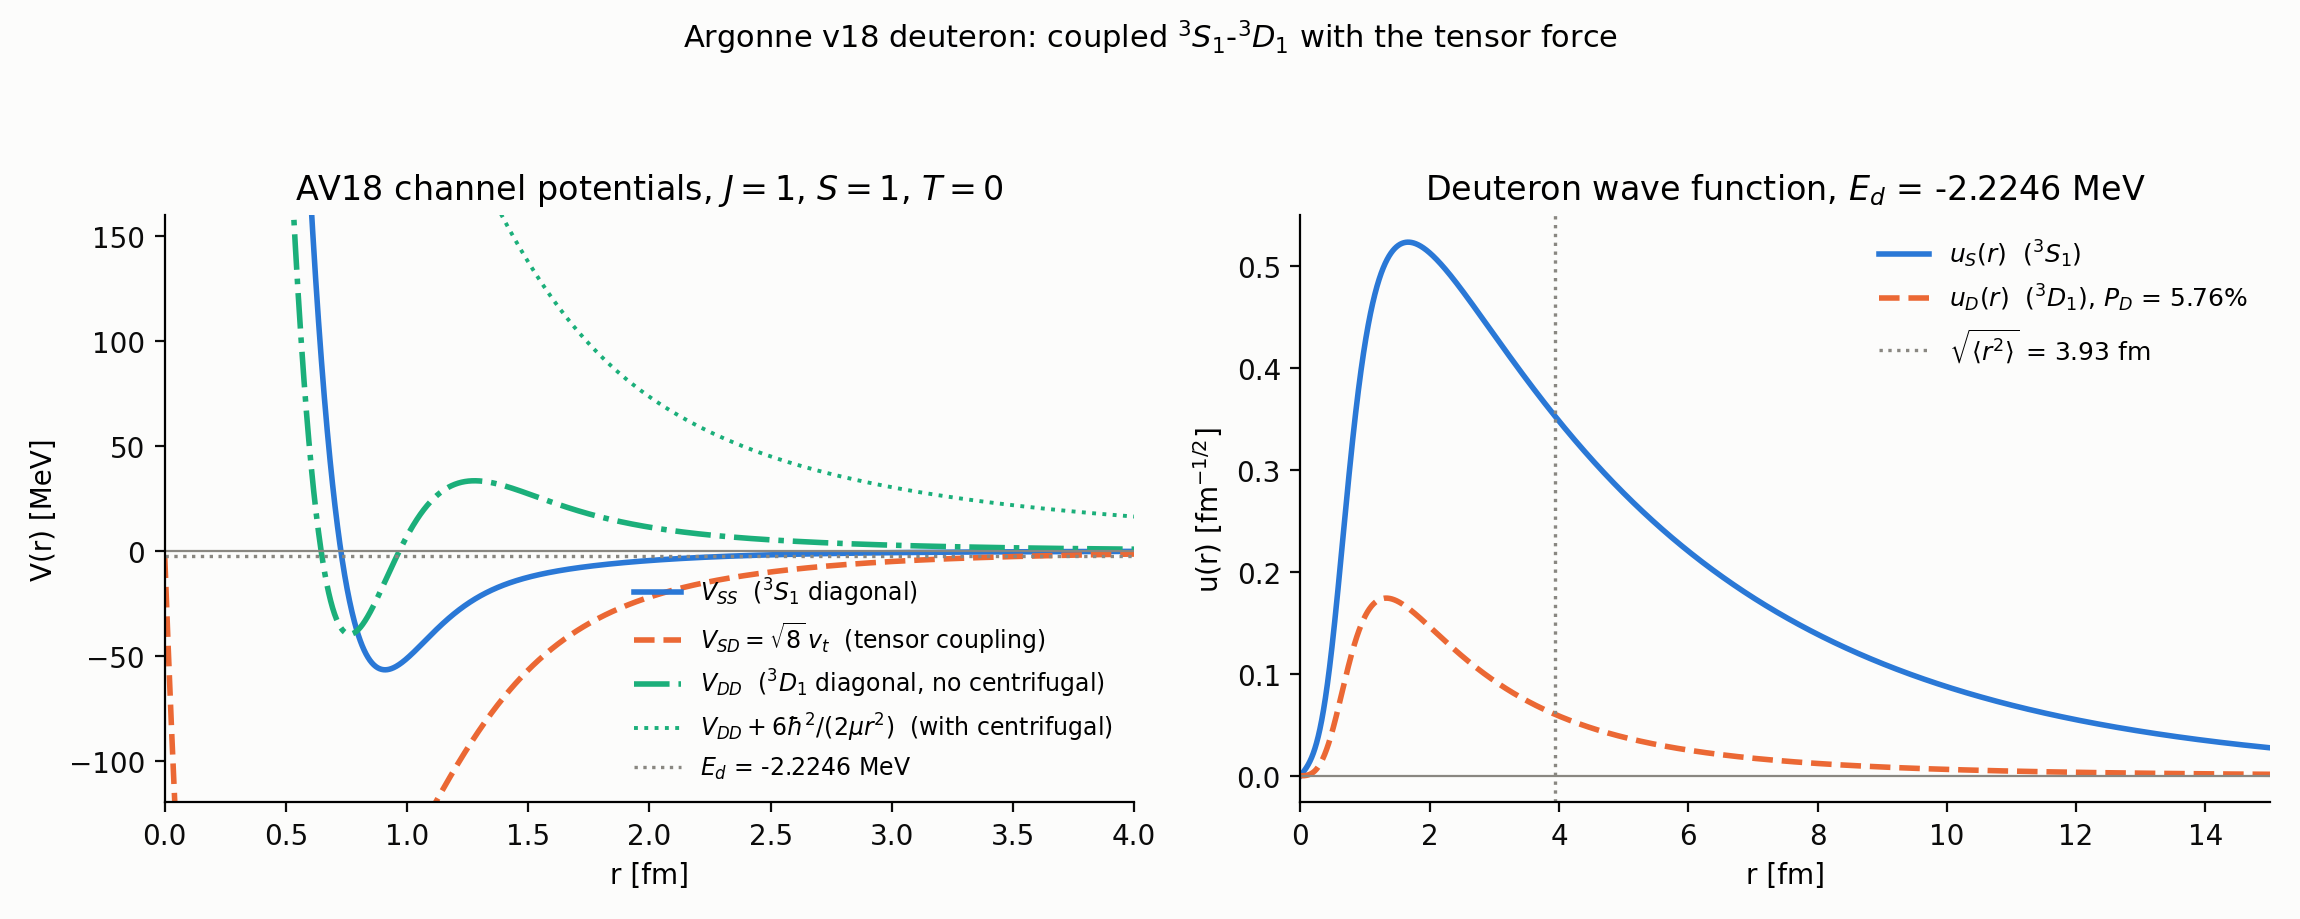
\includegraphics[width=1.0\linewidth]{av18_deuteron.png}
    \caption{Radial dependences of Argonne v18 realistic potential (left).  Deuteron wave function calculated from Argonnne v18 realistic potential (right). }
    \label{deuteron_square_well}
\end{figure}

\subsubsection*{Matrix elements of \texorpdfstring{$\op S_{12}$}{S12}}

What is $\big(LSJM\big|\op S_{12}\big|L'S'J'M'\big)$? $\op S_{12}$ is a scalar
$\to$ the matrix element cannot depend on $M$. Wigner--Eckart theorem:
\[
\big(LSJM\big|\op S_{12}\big|L'S'J'M'\big)
=\underbrace{\big(J'M'\,00\,|\,JM\big)}_{\delta_{JJ'}\delta_{MM'}}
\frac{1}{\sqrt{2J+1}}\big(LSJ\big\|\op S_{12}\big\|L'S'J'\big).
\]
One can show that
\[
\big[\op S_{12},\op S^2\big]=0
\quad\Rightarrow\quad \psi_{JM}=\psi_{JMS},
\]
i.e.\ the interaction does not mix states with $S=0$ and $S=1$:
\[
\big(LSJM\big|\op S_{12}\big|L'S'J'M'\big)=\delta_{MM'}\delta_{JJ'}\delta_{SS'}\,S_{LL'JS}.
\]
Direct evaluation leads to
\[
\big(011M\big|\op S_{12}\big|011M\big)=0,\qquad
\big(211M\big|\op S_{12}\big|011M\big)=2\sqrt2,\qquad
\big(211M\big|\op S_{12}\big|211M\big)=-2,
\]
\[
\Rightarrow\quad
\begin{aligned}
-\frac{\hbar^2}{2\mu}u_0''+V_C\,u_0+2\sqrt2\,V_T\,u_2&=E\,u_0,\\
-\frac{\hbar^2}{2\mu}u_2''+\Big(V_C+\frac{6\hbar^2}{2\mu r^2}-2V_T\Big)u_2+2\sqrt2\,V_T\,u_0&=E\,u_2 .
\end{aligned}
\]

\subsubsection*{Asymptotic solution}

For $r\gg$ range of the potential:
\[
-\frac{\hbar^2}{2\mu}\tilde u_0''=E\,\tilde u_0,\qquad
-\frac{\hbar^2}{2\mu}\tilde u_2''+\frac{6\hbar^2}{2\mu r^2}\tilde u_2=E\,\tilde u_2 .
\]
With $E=E_d<0$, $\alpha=\frac1\hbar\sqrt{2\mu|E_d|}$:
\[
\tilde u_0=A_0\,e^{-\alpha r},\qquad
\tilde u_2=A_2\,e^{-\alpha r}\Big[\frac{1}{(\alpha r)^2}+\frac{1}{\alpha r}+\frac13\Big].
\]

Finally, one can show that the deuteron wave function can be written in a
compact form:
\[
\psi_{JM}=\frac{1}{\sqrt{4\pi}}\Big(\frac{u_0}{r}+\sqrt{\tfrac18}\,\op S_{12}\,\frac{u_2}{r}\Big)\chi^1_M .
\]

Determination of proper radial dependencies of central $V_C$ and tensor $V_T$ parts of nucleon-nucleon interaction is highly non-trivial. Unfortunately, there are conceptual obstacles which prohibit calculation of nucleon-nucleon force "from scratch", i.e, from underlying theory of strong interactions - QCD. Instead, we can construct various models which are able to reproduce available 2-nucleon data. In fact, accurate calculation of deuteron properties can serve as an benchmark of various interaction modesl. The fitting of "realistic" nucleon-nucleon forces requires, however, additional experimental information, which can be extracted from nucleon-nucleon scattering data. 

%=====================================================================
\section{Scattering at low energies}
%=====================================================================
Let's remind basic formulas from partial wave analysis (decomposition) of scattering amplitute. We consider elastic scattering of particle with wave vector $k$ on a spherically symmetric potential $V(r)$. For such potential we can parametrize scattering amplitude as 
\[
f(\vartheta)=\frac1k\sum_{L=0}^{\infty}(2L+1)\,e^{i\delta_L}\sin\delta_L\,P_L(\cos\vartheta),
\]
where $\delta_L$ is phase shift for partial wave with orbital angular momentum quantum number $L$. 
For a finite-range potential with range $\approx R$ sum and wave vector $k$, the sum can be reduced to finite number of term (partial waves) $\displaystyle\sum_{L=0}^{\infty}\approx\sum_{L=0}^{l_{\max}}$

\begin{center}
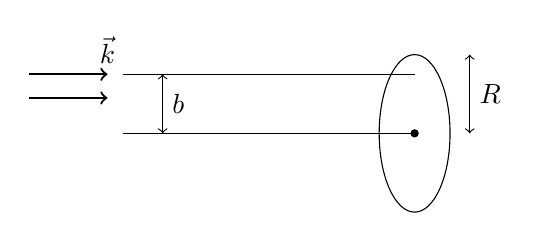
\begin{tikzpicture}[scale=1]
\draw[->,thick] (-0.4,0.75) -- (0.6,0.75) node[above]{$\vec k$};
\draw[->,thick] (-0.4,0.45) -- (0.6,0.45);
\draw (0.8,0.75) -- (4.5,0.75);
\draw (0.8,0) -- (4.5,0);
\draw[<->] (1.3,0) -- (1.3,0.75) node[midway,right]{$b$};
\draw (4.5,0) ellipse (0.45 and 1.0);
\fill (4.5,0) circle (1.5pt);
\draw[<->] (5.2,0) -- (5.2,1.0) node[midway,right]{$R$};
\end{tikzpicture}
\end{center}
with 
\[
l_{\max}\approx R\,\hbar k,\qquad
\hbar\sqrt{\ell_{\max}(\ell_{\max}+1)}\approx R\,\hbar k
\quad\Rightarrow\quad \ell_{\max}\approx Rk .
\]
For small enough energies ($Rk\ll1$), $\ell_{\max}=0$ $\to$ only the $S$-wave
contributes to scattering amplitude
\[
f(\vartheta)\approx\frac1k\,e^{i\delta_0}\sin\delta_0,
\qquad \delta_0 \text{ --- $S$-wave phase shift.}
\]
We define the scattering length $a$ as (for $E\to0$, $k\to0$, $\delta_0\to0$):
\[
a\equiv\lim_{k\to0}\Big[-\frac{\sin\delta_0}{k}\Big]
\quad\Rightarrow\quad
\sigma\approx\int\frac{\ud\sigma}{\ud\Omega}\,\ud\Omega=\int|f|^2\,\ud\Omega
=\frac{4\pi}{k^2}\sin^2\delta_0=4\pi a^2 .
\]

We can determine the scattering length for $p$--$n$ scattering in a simple
square-well model ($m$ is the nucleon mass, $2\mu=m$) which was used before for elementary description of deuteron. 

\begin{center}
\begin{tikzpicture}[scale=1]
\draw[->] (-0.3,1.3) -- (4.0,1.3) node[right]{$r$};
\draw[->] (0,-1.5) -- (0,1.8);
\draw[thick] (0,1.3) -- (0,-1) -- (1.6,-1) -- (1.6,1.3);
\draw[dashed] (0,-1) -- (-0.2,-1) node[left]{$-V_0$};
\node[above] at (1.6,1.3) {$R$};
\node[right] at (4.6,0.2) {$V_0=34\ \text{MeV}$};
\end{tikzpicture}
\end{center}
\[
r\le R:\quad u''+\frac{m}{\hbar^2}(E+V_0)\,u=0,
\qquad\qquad
r\ge R:\quad u''+\frac{m}{\hbar^2}E\,u=0 .
\]
For
\[
r\le R:\quad u(r)=A\sin Kr,\qquad K=\sqrt{\frac{m(E+V_0)}{\hbar^2}},
\]
\[
r\ge R:\quad u(r)=B\sin(kr+\delta),\qquad k=\sqrt{\frac{mE}{\hbar^2}} .
\]
Matching $u'/u$ at $r=R$:
\[
\frac{AK\cos(KR)}{A\sin(KR)}=\frac{Bk\cos(kR+\delta)}{B\sin(kR+\delta)}
\quad\Rightarrow\quad
K\tan(kR+\delta)=k\tan(KR),
\]
\[
K\,\frac{\tan(kR)+\tan\delta}{1-\tan(kR)\tan\delta}=k\tan(KR),
\]
\[
K\big(\tan(kR)+\tan\delta\big)=k\tan(KR)-k\tan(KR)\tan(kR)\tan\delta,
\]
\[
\tan\delta=\frac{k\tan(KR)-K\tan(kR)}{K+k\tan(KR)\tan(kR)}
=\frac{k\Big[\tan(KR)-KR\,\dfrac{\tan(kR)}{kR}\Big]}{K+k\tan(KR)\tan(kR)} .
\]

For small $E$ ($k$):
\[
\delta\approx\frac{k\big[\tan(KR)-KR\big]}{K}=kR\Big(\frac{\tan KR}{KR}-1\Big), 
\]
so for the scattering length we obtain 
\[
a=\lim_{k\to0}\Big[-\frac{\sin\delta}{k}\Big]\approx-\frac{\delta}{k},
\qquad
a\approx R\Big[1-\frac{\tan(KR)}{KR}\Big],
\qquad \sigma=4\pi a^2 .
\]
From the dependence of cross section on $K=\frac{\sqrt{mV_0}}{\hbar}$ is in 
Fig. \ref{resonance_cross_section} we see resonant structure, i.e. for threshold value of well depth cross section diverges to infinity, which corresponds to appearance of bound state. 

\begin{figure}
\begin{center}
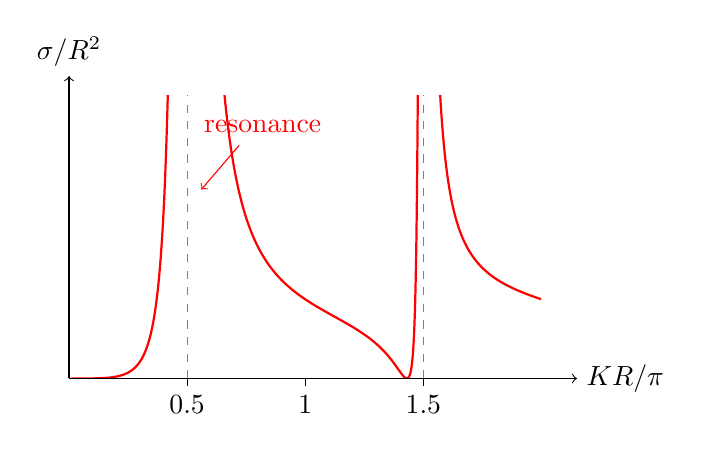
\begin{tikzpicture}[xscale=3,yscale=0.08]
\begin{scope}
\clip (0,0) rectangle (2,45);
\draw[red,thick,domain=0.01:0.497,samples=120,smooth,variable=\t]
  plot ({\t},{4*pi*(min(2.5,abs(1-tan(pi*\t r)/(pi*\t))))^2});
\draw[red,thick,domain=0.503:1.497,samples=200,smooth,variable=\t]
  plot ({\t},{4*pi*(min(2.5,abs(1-tan(pi*\t r)/(pi*\t))))^2});
\draw[red,thick,domain=1.503:2,samples=120,smooth,variable=\t]
  plot ({\t},{4*pi*(min(2.5,abs(1-tan(pi*\t r)/(pi*\t))))^2});
\end{scope}
\draw[->] (0,0) -- (2.15,0) node[right]{$KR/\pi$};
\draw[->] (0,0) -- (0,48) node[above]{$\sigma/R^2$};
\foreach \x in {0.5,1,1.5} \draw (\x,0) -- (\x,-1.2) node[below]{$\x$};
\draw[dashed,gray] (0.5,0) -- (0.5,45);
\draw[dashed,gray] (1.5,0) -- (1.5,45);
\node[red] at (0.82,40) {resonance};
\draw[red,->] (0.72,37) -- (0.56,30);
\end{tikzpicture}
\end{center}
\caption{Resonance structure of S-wave cross section for simple square well potential model.}
\label{resonance_cross_section}
\end{figure}
Let us use $V_0=34$~MeV, then $K=\frac{\sqrt{mV_0}}{\hbar}\doteq0.91\ \text{fm}^{-1}$ and for $R=2.1$~fm gives $a\simeq5.2$~fm and $\sigma\simeq3.4$~b. This is significantly smaller value than experimentally observed value $\sigma^{\rm exp}\simeq20$~b. We would get similar values also for other shapes of potentials which would produce correct bidning energy of deuteron. The argument is similar as before, cross-section for elastic scattering at zero energy is insensitive to to shape of potential, which can be demonstrated by numerical calculation of scattering lenghts for various shapes of potentials.  

This apparent discrepancy lead Wigner to the idea of spin dependence of the $pn$ force. For $pn$ system we have have 2 possibilities:
$S=0$ (singlet) and $S=1$ (triplet). For unpolarized particles total elastic cross section at (nearly) zero energy is a combination of triplet and singlet contributions, with different scattering lenghts $a_t, a_s$, i.e. 
\[
\sigma=\tfrac34\,\sigma_t+\tfrac14\,\sigma_s
\qquad(\sigma_t \text{ --- triplet},\ \sigma_s \text{ --- singlet}).
\]
\[
\sigma_t=4\pi a_t^2,\qquad \sigma_s=4\pi a_s^2.
\]
Experimental data extracted from $pn$ scattering cross section at zero energy are compatible with following values    
\[
\sigma_t=4\pi a_t^2\simeq3.7\ \text{b} ,
\qquad
\sigma_s=4\pi a_s^2\simeq70.6\ \text{b},
\qquad
\sigma\simeq20\ \text{b}.
\]
One can notice that $\sigma_t\simeq3.7$~b is not far from simple estimate based on the square-well potential, whereas value for singlet is much higher, suggesting resonance for singlet case (with no bound state).
%=====================================================================
\subsection{\texorpdfstring{$nH^2$} scattering at low energies}
%=====================================================================
It is clear, that from $pn$ scattering measurement we cannot obtain information about the sign of scattering lenght. 
However, scattering of neutrons on  ortho- and para-H$_2$ can provide additional information. 

Ortho- and para $H^2$ molecules differ by relative orientation of proton spins, wchich can be "paralel" for ortho-$H^2$,and antiparallel for para-$H^2$. This corresponds to $S=1$. i.e spin triplet, or $S=0$, i.e spin singlet state of 2 protons. Because nucleon-nucleon interaction is sensitive to spin orientation, we can use it to determine an unknown signs of scattering lenghts. 
\begin{center}
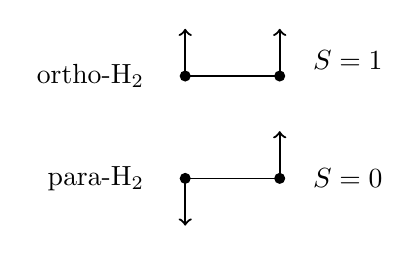
\begin{tikzpicture}[scale=1]
\node[left] at (-0.4,0.3) {ortho-H$_2$};
\fill (0,0.3) circle (2pt); \fill (1.2,0.3) circle (2pt);
\draw (0,0.3) -- (1.2,0.3);
\draw[thick,->] (0,0.3) -- (0,0.9);
\draw[thick,->] (1.2,0.3) -- (1.2,0.9);
\node[right] at (1.5,0.5) {$S=1$};
\node[left] at (-0.4,-1.0) {para-H$_2$};
\fill (0,-1.0) circle (2pt); \fill (1.2,-1.0) circle (2pt);
\draw (0,-1.0) -- (1.2,-1.0);
\draw[thick,->] (0,-1.0) -- (0,-1.6);
\draw[thick,->] (1.2,-1.0) -- (1.2,-0.4);
\node[right] at (1.5,-1.0) {$S=0$};
\end{tikzpicture}
\end{center}

Let us assume scattering of neutron on $H^2$ molecule. If $pn$ scattering can be described by a simple spin-dependent $pn$ potential
\[
\op V=V_0+V_1\,\vec\sigma^{(n)}\!\cdot\vec\sigma^{(p)} , 
\]
then we have effective potentials for singlet and triplet case 
\[
S=0:\quad V_{\rm eff}^{S=0}=V_0-3V_1,
\qquad\qquad
S=1:\quad V_{\rm eff}^{S=1}=V_0+V_1 .
\]
Let us denote
\[
V_S\equiv V_0-3V_1,\qquad V_T\equiv V_0+V_1
\quad\Rightarrow\quad
\tfrac14\big(V_T-V_S\big)=V_1,\qquad
\tfrac14\big(V_S+3V_T\big)=V_0 .
\]

Let us derive the $n$--H$_2$ cross section at low energies
($\lambda_n\gg R_{\rm H_2}$) in terms of the scattering lengths for $n$--$p$
triplet and singlet, determined from $V_T$ and $V_S$.

The $n$--H$_2$ scattering can be described by interaction
\[
\op V_{n\rm H_2}=2V_0+V_1\,\vec\sigma^{(n)}\!\cdot\big(\vec\sigma^{(p_1)}+\vec\sigma^{(p_2)}\big).
\]
Let us introduce
\[
\vec S_{\rm H_2}=\vec s^{\,(p_1)}+\vec s^{\,(p_2)},
\qquad
\vec s^{\,(i)}=\tfrac12\,\vec\sigma^{(i)},\quad i=n,p_1,p_2,
\]
\[
\op V_{n\rm H_2}=\tfrac12\big(V_S+3V_T\big)+\big(V_T-V_S\big)\,\vec s_n\!\cdot\vec S_{\rm H_2} .
\]
We can rewrite the interaction in terms of total spin, neutron spin and spin of $H^2$, i.e. 
\[
\vec S=\vec s_n+\vec S_{\rm H_2},
\qquad
\vec S^{\,2}=\vec s_n^{\,2}+2\,\vec s_n\!\cdot\vec S_{\rm H_2}+\vec S_{\rm H_2}^{\,2},
\]
\[
\op V_{n\rm H_2}=\tfrac12\big(V_S+3V_T\big)
+\big(V_T-V_S\big)\,\tfrac12\Big(\vec S^{\,2}-\vec s_n^{\,2}-\vec S_{\rm H_2}^{\,2}\Big).
\]
We can calculate effective potential for different spin orientations:

Para-$H_2, S_{H_2}=0$
\[
\vec S=\vec s_n+\vec S_{\rm H_2}\quad\Rightarrow\quad S=\tfrac12\quad\text{(doublet)}.
\]
The state is $\ket{\tfrac12\,S_{\rm H_2},\,SM}$ (the first $\tfrac12$ is the
neutron spin), and
\[
V^{\rm eff}_{n\rm H_2}\big(\tfrac12\,S_{\rm H_2}\,S\big)
=\Braket{\tfrac12\,S_{\rm H_2},SM|\op V_{n\rm H_2}|\tfrac12\,S_{\rm H_2},SM}
\]
\begin{align*}
\Rightarrow\quad
V^{\rm eff}_{n\rm H_2}\big(\tfrac12\,0\,\tfrac12\big)
&=\Braket{\tfrac12\,0,\tfrac12M|\op V_{n\rm H_2}|\tfrac12\,0,\tfrac12M}\\
&=\tfrac12\big(V_S+3V_T\big)+\big(V_T-V_S\big)\,\tfrac12\Big(\tfrac12\big(\tfrac12+1\big)
-\tfrac12\big(\tfrac12+1\big)-0\,(0+1)\Big)\\
&=\tfrac12\big(V_S+3V_T\big).
\end{align*}

Ortho-$H_2, S_{\rm H_2}=1$
\[
S=\tfrac12+1\ \Big\langle\
\begin{matrix}\tfrac12\\[1mm]\tfrac32\end{matrix}
\]

$S=\tfrac12$ (doublet):
\begin{align*}
V^{\rm eff}_{n\rm H_2}&=\tfrac12\big(V_S+3V_T\big)+\big(V_T-V_S\big)\,\tfrac12
\Big[\tfrac12\big(\tfrac12+1\big)-\tfrac12\big(\tfrac12+1\big)-1(1+1)\Big]\\
&=\tfrac12\big(V_S+3V_T\big)-\big(V_T-V_S\big)
=\tfrac12V_T+\tfrac32V_S. 
\end{align*}

$S=\tfrac32$ (quartet):
\begin{align*}
V^{\rm eff}_{n\rm H_2}&=\tfrac12\big(V_S+3V_T\big)+\big(V_T-V_S\big)\,\tfrac12
\Big[\tfrac32\big(\tfrac32+1\big)-\tfrac12\big(\tfrac12+1\big)-1(1+1)\Big]\\
&=\tfrac12\big(V_S+3V_T\big)+\tfrac12\big(V_T-V_S\big)=2V_T .
\end{align*}

So we have 3 types of interaction:
\begin{center}
\renewcommand{\arraystretch}{1.5}
\begin{tabular}{l l l}
para-H$_2$ & $S=\tfrac12$ (doublet) & $V^{\rm eff}=\tfrac12\big(V_S+3V_T\big)$ \\
ortho-H$_2$ & $S=\tfrac12$ (doublet) & $V^{\rm eff}=\tfrac12V_T+\tfrac32V_S$ \\
 & $S=\tfrac32$ (quartet) & $V^{\rm eff}=2V_T$
\end{tabular}
\end{center}
If we assume, that for effective triplet interaction $V_T$ cooresponding scattering lenght is $a_t$, and for effective singlet interaction $V_S$ it is $a_s$, we can write for the cross section 
\[
\sigma_{\rm para}=4\pi\Big(\tfrac32\,a_t+\tfrac12\,a_s\Big)^2=\pi\big(3a_t+a_s\big)^2,
\]
\[
\sigma_{\rm ortho}=4\pi\Big[\tfrac23\big(2a_t\big)^2
+\tfrac13\Big(\tfrac12\,a_t+\tfrac32\,a_s\Big)^2\Big]
=\pi\Big[\big(3a_t+a_s\big)^2+2\big(a_t-a_s\big)^2\Big].
\]
The weights $\tfrac23$, $\tfrac13$ in the case of ortho-hydrogen follow from the number of states (spin projections), i.e. $\text{quartet} : \text{doublet} \rightarrow 4:2=2:1$.
One can also notice that $\sigma_{\rm ortho}\gg\sigma_{\rm para}$.


In reality, the dependence of the cross section is more complicated, for example due to the molecular effects, but it can be parametrized as
\[
\sigma=c_1\big(a_t-a_s\big)^2+c_2\big(3a_t+a_s\big)^2,
\]
where the coefficients depend on the incident energy, temperature, \dots, and
are different for ortho- and para-hydrogen. This allows for the exctraction of singlet and triplet scattering lenghts 
Experimental data are compatible with following values of scattering lenghts for triplet and singlet.   
\[
a_t\simeq5.4\ \text{fm},\qquad a_s\simeq-23.7\ \text{fm}.
\]
We see that positive sign for triplet supports the existence of a bound state (deuteron), whereas singlet confuguration is unboud. 


In the case of $pp$ scattering situation is more complicated due to the long-range Coulomb
interaction, and the particles are identical:
\[
\frac{\ud\sigma}{\ud\Omega}\sim\big|f(\vartheta,\varphi)+f(\pi-\vartheta,\pi+\varphi)\big|^2 .
\]

\begin{center}
\begin{tikzpicture}[scale=1]
% direct
\draw (0,1.5) -- (1.8,1.5);
\draw[->] (1.8,1.5) -- (2.6,1.95);
\draw (2.6,1.95) -- (3.4,2.4);
\draw (4.0,1.6) -- (2.2,1.6);
\draw[->] (2.2,1.6) -- (1.5,0.95);
\draw (1.5,0.95) -- (0.8,0.3);
% exchange
\begin{scope}[xshift=5cm]
\draw (0,1.5) -- (1.9,1.5) .. controls (2.3,1.5) and (2.2,1.1) .. (1.7,0.8);
\draw[->] (1.7,0.8) -- (1.2,0.45);
\draw (1.2,0.45) -- (0.6,0.1);
\draw (4.2,1.5) -- (2.5,1.5) .. controls (2.1,1.5) and (2.4,1.9) .. (2.8,2.1);
\draw[->] (2.8,2.1) -- (3.2,2.35);
\draw (3.2,2.35) -- (3.6,2.6);
\end{scope}
\end{tikzpicture}
\end{center}

Because we deal with identical fermions, wave function must by antisymmetric with respect to exchagne of particles, which leads to restrictions for combination of angular and spin part
\[
L=0,2,4,\dots:\ \chi^0,\qquad\qquad L=1,3,5,\dots:\ \chi^1 .
\]
Total scattering amplitude is composed of Coulomb part $fˆC$ and nuclear part $fˆN$
\[
f=f^C+f^N\qquad(f^C \text{ --- Coulomb part},\ f^N \text{ --- nuclear part}),
\]
and cross section can be split to Coulomb, nuclear and "interference" terms. 
\[
\frac{\ud\sigma}{\ud\Omega}=\Big(\frac{\ud\sigma}{\ud\Omega}\Big)_C
+\Big(\frac{\ud\sigma}{\ud\Omega}\Big)_N
+\Big(\frac{\ud\sigma}{\ud\Omega}\Big)_{CN}
\quad(\to \text{interference term}),
\]
\[
\Big(\frac{\ud\sigma}{\ud\Omega}\Big)_N\approx\frac{\sin^2\delta_0}{k^2}
\qquad\text{for small energies.}
\]

%=====================================================================
\subsection{Effective range}
%=====================================================================

Let us go back to $p$--$n$ scattering. We can derive approximate formula for the cross section for $S$ scattering for small (non-zero) energies which is valid up to $\approx$ 10 MeV, in the literature known as effective range expansion. 

The S-wave phase shift can be determined from the asymptotic solution for $\ell=0$
\[
\bar u_{k_0}=r\,\bar R_{k_0}=A\sin(kr+\delta_0).
\]

For 2 different energies (small enough), $E_1>0$, $E_2>0$ we denote corresponding solutions $u_1, u_2$.
\[
\begin{aligned}
u_1''+\frac{m}{\hbar^2}\big(E_1-V(r)\big)\,u_1&=0,\\
u_2''+\frac{m}{\hbar^2}\big(E_2-V(r)\big)\,u_2&=0,
\end{aligned}
\qquad\qquad
E_i=\frac{\hbar^2k_i^2}{2\mu},\quad i=1,2,\qquad \mu\simeq\frac m2 .
\]
Further, for bound states (deuteron), $E_d<0$:
\[
u_d''+\frac{m}{\hbar^2}\big(E_d-V(r)\big)\,u_d=0 .
\]
We require boundary conditions
\[
u_1(0)=u_2(0)=u_d(0)=0
\]
and asymptotic solutions ($r\to\infty$, $r\gg R$):
\[
u_1\to\bar u_1,\qquad u_2\to\bar u_2,\qquad u_d\to\bar u_d .
\]

Multiplying the first equation by $u_2$ and the second by $u_1$:
\[
\begin{aligned}
u_2\,u_1''+\frac{m}{\hbar^2}\big(E_1-V\big)\,u_1u_2&=0,\\
u_1\,u_2''+\frac{m}{\hbar^2}\big(E_2-V\big)\,u_1u_2&=0,
\end{aligned}
\]
\[
\text{and performing integration} 
\Rightarrow\quad
\int_0^\infty\!\ud r\,\big(u_2u_1''-u_1u_2''\big)
+\frac{m}{\hbar^2}\big(E_1-E_2\big)\int_0^\infty\!\ud r\,u_1u_2=0,
\]
where
\[
\int_0^\infty\!\ud r\,\big(u_2u_1''-u_1u_2''\big)
=\int_0^\infty\!\ud r\,\frac{\ud}{\ud r}\big(u_2u_1'-u_1u_2'\big)
=\Big[u_2u_1'-u_1u_2'\Big]_0^\infty
\]
\[
\Rightarrow\quad
\Big[u_2u_1'-u_1u_2'\Big]_0^\infty=\frac{m}{\hbar^2}\big(E_2-E_1\big)\int_0^\infty\!\ud r\,u_1u_2 .
\]
The same equation is valid for $\bar u$:
\[
\Big[\bar u_2\bar u_1'-\bar u_1\bar u_2'\Big]_0^\infty
=\frac{m}{\hbar^2}\big(E_2-E_1\big)\int_0^\infty\!\ud r\,\bar u_1\bar u_2
\]
Subtruction of those equations gives 
\[
\Big[u_2u_1'-u_1u_2'-\bar u_2\bar u_1'+\bar u_1\bar u_2'\Big]_0^\infty
=\frac{m}{\hbar^2}\big(E_2-E_1\big)\int_0^\infty\!\ud r\,\big(u_1u_2-\bar u_1\bar u_2\big).
\]
If we assume that $u_1(0)=u_2(0)=0$, derivatives $u_1'(0)$, $u_2'(0)$ do not diverge, and $u_i(\infty)\to\bar u_i$ we get 
\[
\bar u_2(0)\,\bar u_1'(0)-\bar u_1(0)\,\bar u_2'(0)
=\frac{m}{\hbar^2}\big(E_2-E_1\big)\int_0^\infty\big(u_1u_2-\bar u_1\bar u_2\big)\,\ud r .
\]

With
\[
\bar u_i=A_i\sin(k_ir+\delta_i),\qquad \delta_i\equiv\delta_0(E_i),
\]
\[
\bar u_2\bar u_1'-\bar u_1\bar u_2'
=A_2\sin(k_2r+\delta_2)\,A_1k_1\cos(k_1r+\delta_1)
-A_1\sin(k_1r+\delta_1)\,A_2k_2\cos(k_2r+\delta_2).
\]
from which we get (for $r=0$)
\begin{multline*}
A_1A_2\big(k_1\sin\delta_2\cos\delta_1-k_2\sin\delta_1\cos\delta_2\big)\\
=\frac{m}{\hbar^2}\big(E_2-E_1\big)\int_0^\infty\big(u_1u_2-\bar u_1\bar u_2\big)\,\ud r
\qquad\Big/\cdot\ \frac{1}{A_1A_2\sin\delta_1\sin\delta_2}\equiv N
\end{multline*}
\[
k_1\cot\delta_1-k_2\cot\delta_2
=\frac{m}{\hbar^2}\big(E_2-E_1\big)\,N\int_0^\infty\big(u_1u_2-\bar u_1\bar u_2\big)\,\ud r .
\]
(\emph{Note:} $A_1$, $A_2$ can be chosen so that $N=1$.)

The integral $N\int_0^\infty\big(u_1u_2-\bar u_1\bar u_2\big)\,\ud r$ is unknown.
It is common to define the function
\[
\rho(E_1,E_2)=2N\int_0^\infty\big(\bar u_1\bar u_2-u_1u_2\big)\,\ud r,
\]
\[
\Rightarrow\quad
k_1\cot\delta_1-k_2\cot\delta_2=\frac{m}{2\hbar^2}\big(E_1-E_2\big)\,\rho(E_1,E_2).
\]

Since
\[
k\cot\delta=k\,\frac{\cos\delta}{\sin\delta}\ \xrightarrow{\;k\to0\;}\ -\frac1a,
\qquad
a\equiv\lim_{k\to0}\Big[-\frac{\sin\delta}{k}\Big],
\]
we set $k_1\equiv k$, $\delta_1\equiv\delta$, $E_1\equiv E$, and $E_2\to0$:
\[
k\cot\delta+\frac1a=\frac{m}{2\hbar^2}\,E\,\rho(E,0),
\qquad
\rho(E,0)=2N\int_0^\infty\big(\bar u\,\bar u_0-u\,u_0\big)\,\ud r,
\]
with $u$ the solution for $E$ and $u_0$ the solution for $E\to0$.

It turns out that $\rho(E,0)$ changes slowly with $E$ for small $E$:
\[
\rho(E,0)\approx\rho(0,0)\equiv r_{\rm eff},
\]
\[
\boxed{\;k\cot\delta+\frac1a\simeq\frac12\,k^2\,r_{\rm eff}\;}
\qquad\qquad
E=\frac{\hbar^2k^2}{2\mu}=\frac{\hbar^2k^2}{m},\quad \mu=\frac m2,
\]
The quantity  $r_{\rm eff}$ is called  "effective range" .
The cross section for elastic scattering at low energies can be then expressed as
\[
\sigma=\frac{4\pi}{k^2}\sin^2\delta=\frac{4\pi}{k^2}\,\frac{1}{1+\cot^2\delta}
=\frac{4\pi}{k^2}\,\frac{1}{1+\frac{1}{k^2}\big(\frac12k^2r_{\rm eff}-\frac1a\big)^2}
\]
\[
\boxed{\;\sigma=\frac{4\pi a^2}{k^2a^2+\big(1-\frac12\,a\,k^2\,r_{\rm eff}\big)^2}\;}
\]
The cross section is given by 2 parameters $a$, $r_{\rm eff}$, which for an unknown potential can be determined by fitting to experimental data. For low energies, this parameters do not depend much on actual shape of the potential, because large wave length of scattering particle does not allow to probe details of potential.



Moreover, because the interaction depends on spin orientation we have different scattering lenghts and effective ranges for triplet $a_t, r_t$ and singlet $a_s,r_s$. The cross section is then given by
\[
\;\sigma=\frac{3}{4} \frac{4\pi a_t^2}{k^2a_t^2+\big(1-\frac12\,a_t\,k^2\,r_t\big)^2}\ +
\frac{1}{4} \frac{4\pi a_s^2}{k^2a_s^2+\big(1-\frac12\,a_s\,k^2\,r_s\big)^2}.
\]

The comparison of data with the formula based on effective range expansion is on Fig. \ref{pn_crs_low_en}.
\begin{figure}
    \centering
    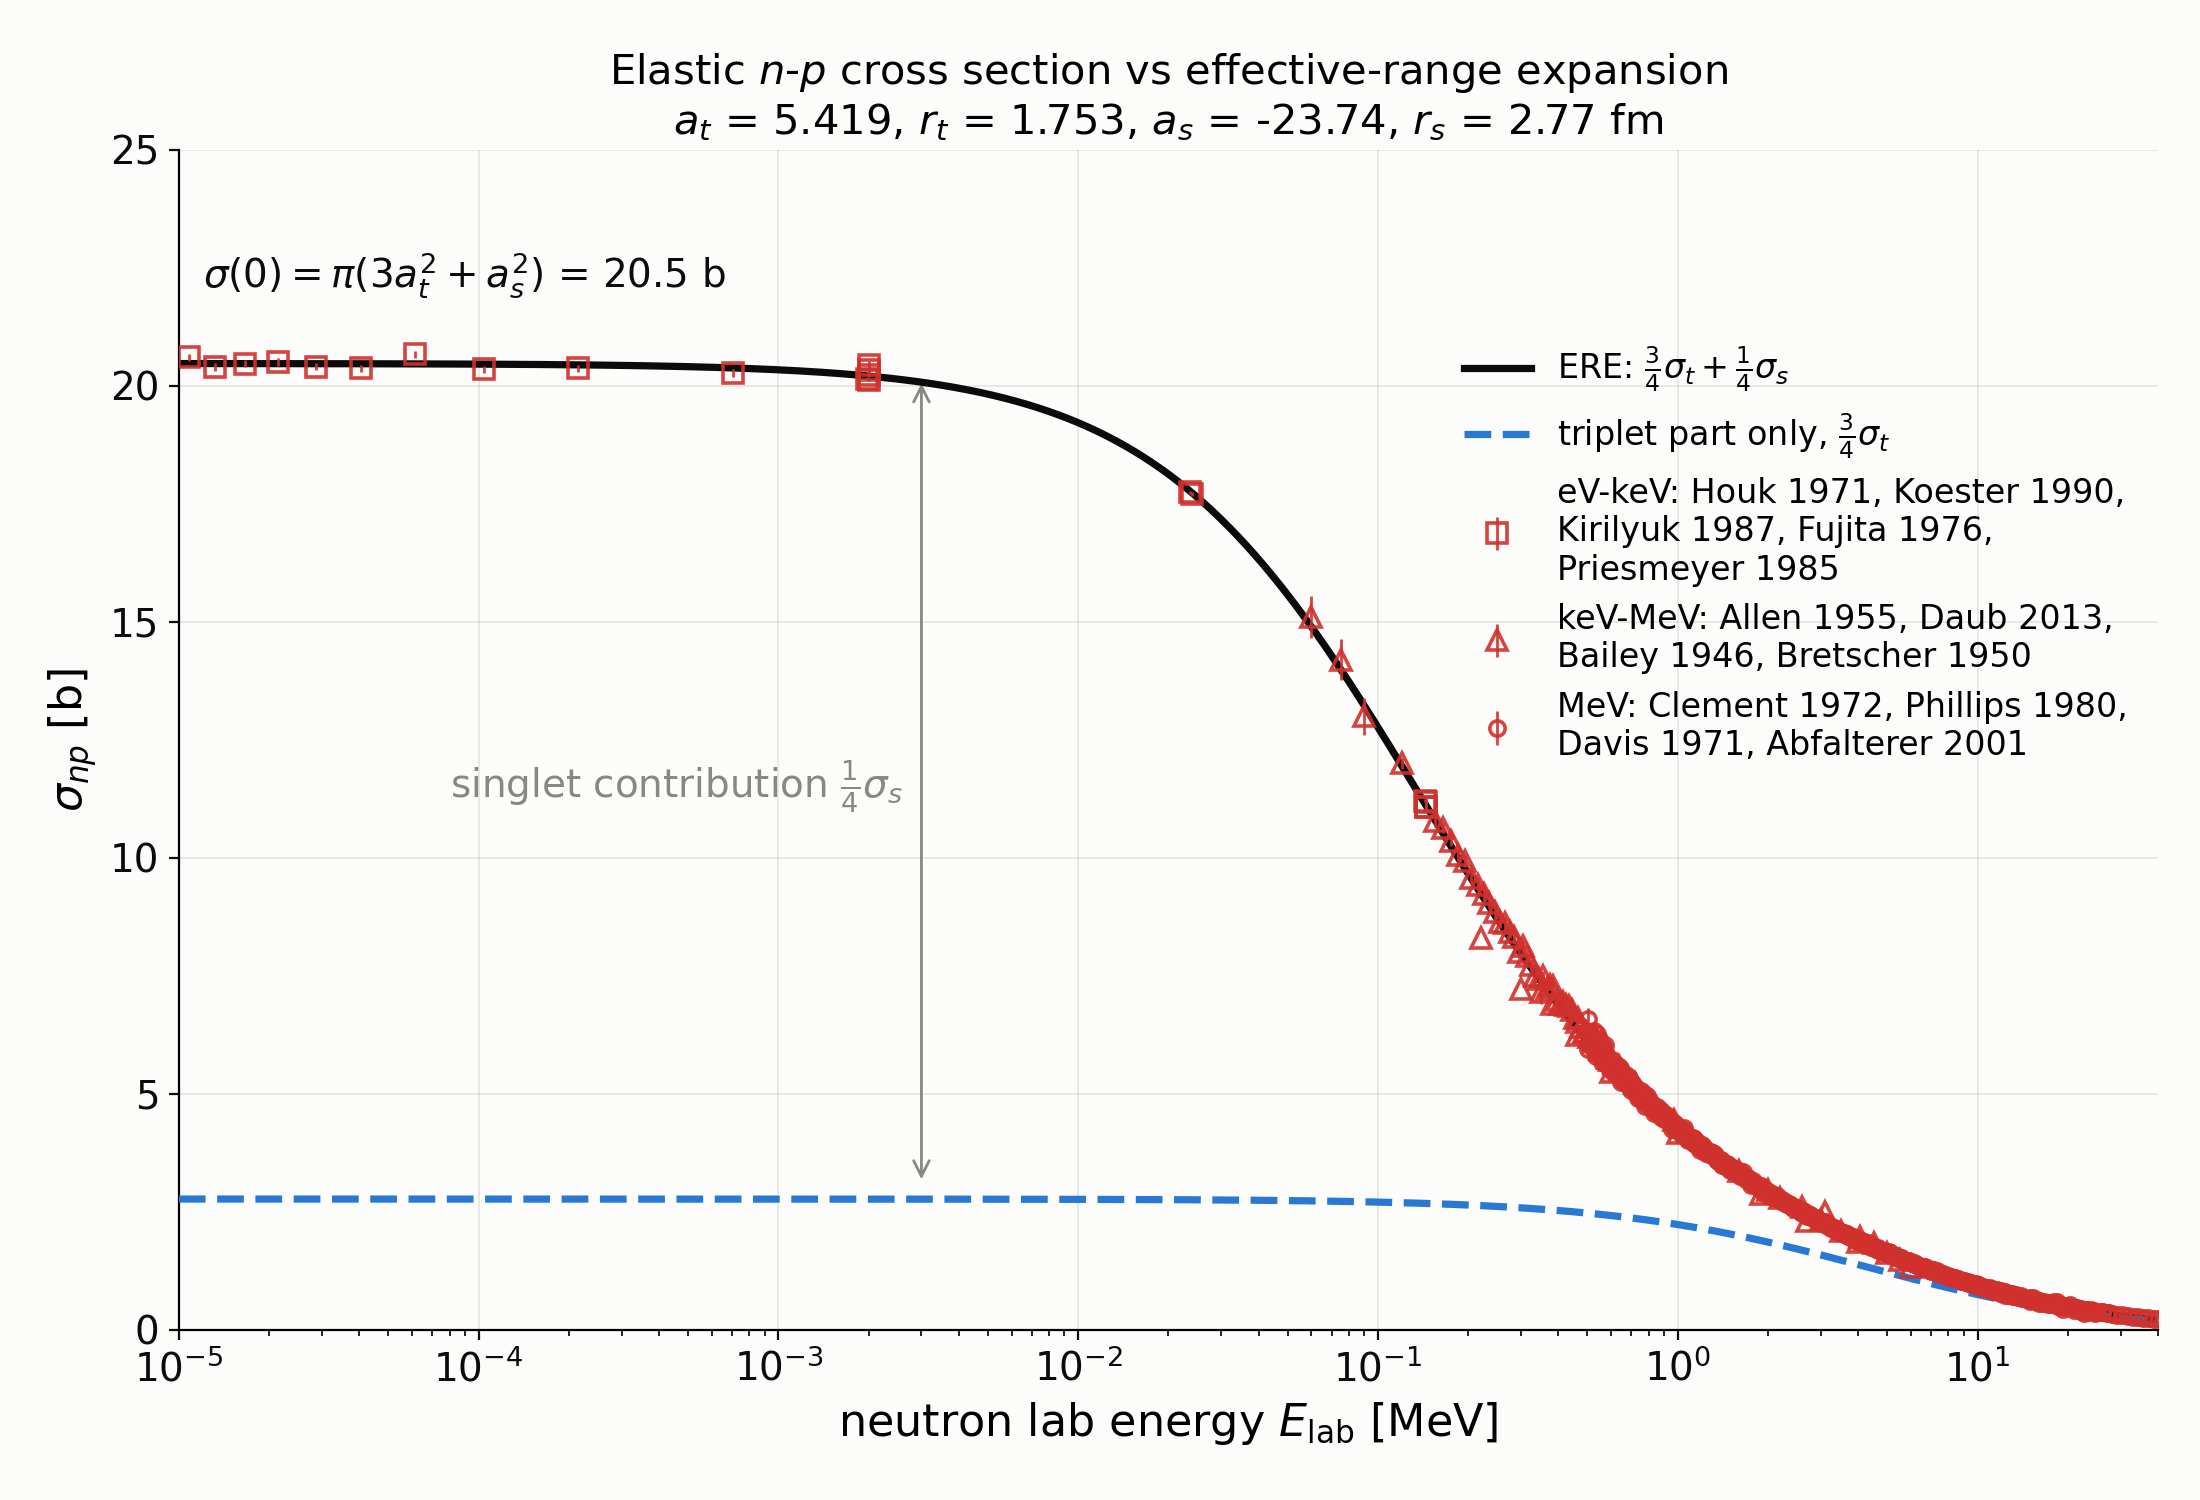
\includegraphics[width=0.8\linewidth]{np_cross_section_ere.png}
    \caption{Elastic scattering cross-section for $pn$ scattering for low energies.}
    \label{pn_crs_low_en}
\end{figure}


\subsection{Higher partial waves}

To get information about the details of the potential, we have to include
higher partial waves, $\ell>0$. Starting from
\[
f(\vartheta)=\frac1k\sum_{\ell=0}^{\infty}(2\ell+1)\,e^{i\delta_\ell}\sin\delta_\ell\,P_\ell(\cos\vartheta).
\]
Let's assume next term, i.e. $\ell=0,1$:
\[
f(\vartheta)=\frac1k\,e^{i\delta_0}\sin\delta_0+\frac1k\,3\,e^{i\delta_1}\sin\delta_1\cos\vartheta ,
\]
\[
|f(\vartheta)|^2=|f_0+f_1|^2=|f_0|^2+|f_1|^2+2\,\mathrm{Re}\big(f_0^*f_1\big),
\]
\[
f_0^*f_1=\frac{1}{k^2}\,3\,e^{i(\delta_1-\delta_0)}\sin\delta_0\sin\delta_1\cos\vartheta,
\qquad
\mathrm{Re}\big(f_0^*f_1\big)=\frac{1}{k^2}\,3\cos(\delta_1-\delta_0)\sin\delta_0\sin\delta_1\cos\vartheta,
\]
\[
\frac{\ud\sigma}{\ud\Omega}=\frac{1}{k^2}\Big(
\underbrace{\sin^2\delta_0}_{\ell=0}+\underbrace{9\sin^2\delta_1\cos^2\vartheta}_{\ell=1}
+\underbrace{6\cos(\delta_1-\delta_0)\sin\delta_0\sin\delta_1\cos\vartheta}_{\text{interf.\ term}}\Big).
\]
We see that cross section now includes also angular dependence. Inclusion of higher partial waves leads to more complicated, expressions. In fact, we can understand partial wave expansion as parametrisation of elastic cross section in terms of phase shift parameters. 

Determination of phase shifts from data is essentially a nontrivial, but well defined, fitting procedure. Phase shifts for relevant $S,T,L$ channels can be used in construction of realistic NN potentials, in particular for restriction of an unknown radial (or momentum) dependencies. Let us note, that another complication comes from the existence of tensor force, which mixes partial waves with different $L$, therefore partial wave analysis is more complicated as presented here. However, an extension of partial wave method which includes such mixing can be formulated, and, therefore phase shifts can be determined for realistic interactions.

Usually experimetal data up to $\approx 350 MeV$ are taken into account in partial wave analysis of NN scattering. For energies larger than $290$~MeV in the lab, ( i.e. $140$~MeV in the CM frame) production of $\pi$ mesons is possible, i.e. an inelastic processes start to contribute.  

%=====================================================================
\subsection{Operatorial structure of \texorpdfstring{$NN$}{NN} interaction}
%=====================================================================

\begin{itemize}
\item nucleonic degrees of freedom,
\item non-relativistic QM.
\end{itemize}

\[
\vec r,\ \vec p \ \text{--- relative coordinate and momentum},\qquad
\vec\sigma^{(1)},\ \vec\sigma^{(2)} \ \text{--- spins},\qquad
\vec\tau^{(1)},\ \vec\tau^{(2)} \ \text{--- isospins}.
\]

Symmetries:
\[
\op V=\op V^\dagger,\qquad
V(1,2)=V(2,1),\qquad
V(\vec r,\dots),\ V(\vec p,\dots)\ \text{(relative coordinates only)},
\]
\[
V(\vec r,\vec p,\dots)=V(-\vec r,-\vec p,\dots),\qquad
V(\vec r,\vec p,\vec\sigma,\dots)=V(\vec r,-\vec p,-\vec\sigma,\dots),\qquad
\text{rotational invariance}.
\]

\subsection{Local potentials}

Local potentials $\to$ no dependence on $\vec p$.

Spin-dependent part:
\[
\vec\sigma^{(1)}\!\cdot\vec\sigma^{(2)} .
\]
$\vec r\cdot\vec\sigma^{(1)}$ is a pseudoscalar. But
\[
\big(\vec\sigma^{(1)}\!\cdot\vec r\big)\big(\vec\sigma^{(2)}\!\cdot\vec r\big)
\quad\text{is a scalar --- ``tensor force''.}
\]
Conventionally we use
\[
\op S_{12}=3\big(\vec\sigma^{(1)}\!\cdot\vec n\big)\big(\vec\sigma^{(2)}\!\cdot\vec n\big)
-\big(\vec\sigma^{(1)}\!\cdot\vec\sigma^{(2)}\big),
\qquad \vec n=\frac{\vec r}{r},
\]
satisfying
\[
\int\!\ud\Omega\,\op S_{12}=0 .
\]

A general spin-dependent interaction contains the terms
\[
\op V=\underbrace{U_c(r)}_{\text{central}}
+\underbrace{U_\sigma\,\big(\vec\sigma^{(1)}\!\cdot\vec\sigma^{(2)}\big)}_{\text{spin}}
+\underbrace{U_t\,\op S_{12}}_{\text{tensor}} .
\]

\subsubsection*{Spin exchange operator}

\[
\op P^\sigma=\tfrac12\big(\mathbf 1+\vec\sigma^{(1)}\!\cdot\vec\sigma^{(2)}\big)
\qquad\text{--- spin exchange operator (Bartlett operator)},
\]
\[
\big[\op P^\sigma,\op V\big]=0
\quad\Rightarrow\quad
\text{spin triplet and singlet states cannot mix.}
\]

\subsection{Isospin degrees of freedom}

Isospin degrees of freedom $\to$ $\vec\tau^{(1)}\!\cdot\vec\tau^{(2)}$ terms.

Isotropic part of the potential:
\[
U_c(r)+U_\sigma\big(\vec\sigma^{(1)}\!\cdot\vec\sigma^{(2)}\big)
+U_{c\tau}\big(\vec\tau^{(1)}\!\cdot\vec\tau^{(2)}\big)
+U_{\sigma\tau}\big(\vec\sigma^{(1)}\!\cdot\vec\sigma^{(2)}\big)\big(\vec\tau^{(1)}\!\cdot\vec\tau^{(2)}\big).
\]

Pauli principle:
\[
\op P^r\,\op P^\sigma\,\op P^\tau=-1 ,
\]
with the exchange operators
\[
\op P^r:\ \vec r_1\leftrightarrow\vec r_2,\quad
\op P^r\,\psi(\vec r_1,\vec r_2)=\psi(\vec r_2,\vec r_1),
\qquad
\op P^\sigma=\tfrac12\big(\mathbf 1+\vec\sigma^{(1)}\!\cdot\vec\sigma^{(2)}\big),
\qquad
\op P^\tau=\tfrac12\big(\mathbf 1+\vec\tau^{(1)}\!\cdot\vec\tau^{(2)}\big).
\]

Concerning the tensor force $\op S_{12}$: $\ \op S_{12}\,\vec\sigma^{(1)}\!\cdot\vec\sigma^{(2)}$
does not bring a new term, therefore
\[
U_t\,\op S_{12}+U_{t\tau}\,\op S_{12}\,\vec\tau^{(1)}\!\cdot\vec\tau^{(2)} .
\]

\subsection{General local interaction}

The general local interaction therefore is
\begin{multline*}
\op V=U_c+U_\sigma\,\vec\sigma^{(1)}\!\cdot\vec\sigma^{(2)}
+U_{c\tau}\,\vec\tau^{(1)}\!\cdot\vec\tau^{(2)}
+U_{\sigma\tau}\big(\vec\sigma^{(1)}\!\cdot\vec\sigma^{(2)}\big)\big(\vec\tau^{(1)}\!\cdot\vec\tau^{(2)}\big)\\
+U_t\,\op S_{12}+U_{t\tau}\,\op S_{12}\,\vec\tau^{(1)}\!\cdot\vec\tau^{(2)}
\end{multline*}
\[
\Rightarrow\quad U_c,\ U_\sigma,\ U_{c\tau},\ U_{\sigma\tau},\ U_t,\ U_{t\tau}
\quad\to\quad 6 \text{ radial functions},
\]
fitted to scattering data and the deuteron.

\subsection{Argonne potentials}

An example is the family of Argonne potentials.

\textbf{Argonne $v_4$} --- only the isotropic part:
\[
\begin{aligned}
V^{\rm eff}(S=1,\,T=0)&=U_c+U_\sigma-3\big(U_{c\tau}+U_{\sigma\tau}\big),\\
V^{\rm eff}(S=0,\,T=1)&=U_c-3U_\sigma+U_{c\tau}-3U_{\sigma\tau},
\end{aligned}
\]
which can easily be shown with the help of
\[
\begin{aligned}
\vec\sigma^{(1)}\!\cdot\vec\sigma^{(2)}\ket{S=0}&=-3\ket{S=0},&\qquad
\vec\tau^{(1)}\!\cdot\vec\tau^{(2)}\ket{T=0}&=-3\ket{T=0},\\
\vec\sigma^{(1)}\!\cdot\vec\sigma^{(2)}\ket{S=1}&=\ket{S=1},&\qquad
\vec\tau^{(1)}\!\cdot\vec\tau^{(2)}\ket{T=1}&=\ket{T=1}.
\end{aligned}
\]

\subsubsection*{Radial shape}

Short-range character ($r>2$~fm weak), repulsive core ($r\lesssim0.7$~fm).

\begin{center}
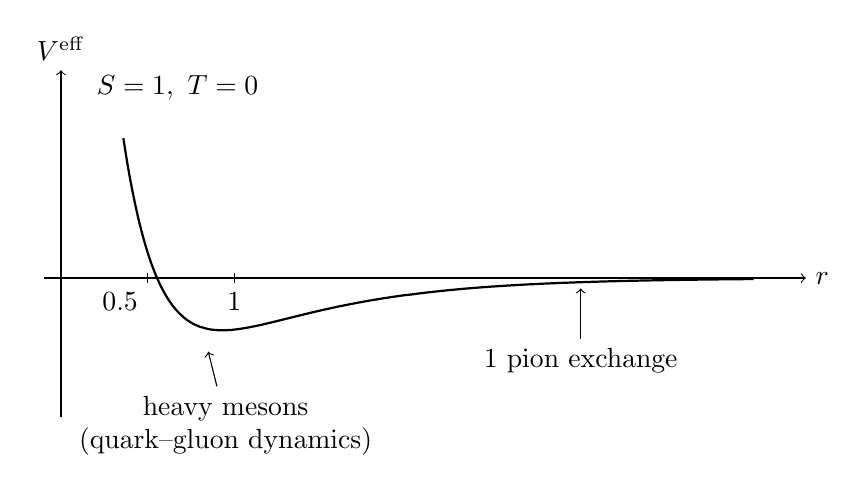
\begin{tikzpicture}[xscale=2.2,yscale=1.1]
\draw[->] (-0.1,0) -- (4.3,0) node[right]{$r$};
\draw[->] (0,-1.6) -- (0,2.4) node[above]{$V^{\rm eff}$};
\node[right] at (0.15,2.2) {$S=1,\ T=0$};
\draw (0.5,0.06) -- (0.5,-0.06) node[below left]{$0.5$};
\draw (1,0.06) -- (1,-0.06) node[below]{$1$};
\draw[thick,domain=0.36:4,samples=200,smooth]
  plot (\x,{min(2.3, 18*exp(-4.5*\x) - 1.6*exp(-1.4*(\x-0.5)))});
\draw[->] (0.9,-1.25) -- (0.85,-0.85);
\node[below,align=center] at (0.95,-1.25)
  {heavy mesons\\(quark--gluon dynamics)};
\draw[->] (3.0,-0.7) -- (3.0,-0.12);
\node[below] at (3.0,-0.7) {1 pion exchange};
\end{tikzpicture}
\end{center}

\textbf{Soft core} $\to$ phenomenological $\to$ incorporates complicated
physics at short distances:
\[
U_{sc}=\frac{C}{1+e^{(r-r_c)/a_c}},\qquad r_c=0.5\ \text{fm},\quad a_c=0.2\ \text{fm},
\]
\[
U_{sc}(r=0)\approx C,\qquad U_{sc}(r=r_c)=C/2,
\]
$C=2$~GeV! for the central part $\to$ very strong repulsion.

\begin{center}
\begin{tikzpicture}[xscale=2.0,yscale=1.0]
\draw[->] (-0.1,0) -- (2.2,0) node[right]{$r$};
\draw[->] (0,-0.2) -- (0,2.4) node[above]{$U_{sc}$};
\draw[thick,domain=0:2.0,samples=150,smooth]
  plot (\x,{2/(1+exp((\x-0.5)/0.2))});
\draw[dashed] (0.5,0) -- (0.5,1) -- (0,1) node[left]{$C/2$};
\node[left] at (0,2) {$C$};
\node[below] at (0.5,0) {$r_c$};
\end{tikzpicture}
\end{center}

\subsection{Additional terms}

\[
\vec L\cdot\vec S=\big(\vec r\times\vec p\big)\cdot\vec S\qquad\text{(non-local)},
\]
\[
U_{LS}\,\vec L\cdot\vec S,\qquad
U_{LS\tau}\,\vec L\cdot\vec S\,\big(\vec\tau^{(1)}\!\cdot\vec\tau^{(2)}\big).
\]

Higher terms:
\[
\vec L^{\,2},\qquad
\vec L^{\,2}\big(\vec\sigma^{(1)}\!\cdot\vec\sigma^{(2)}\big),\qquad
\vec L^{\,2}\big(\vec\tau^{(1)}\!\cdot\vec\tau^{(2)}\big),\qquad
\vec L^{\,2}\big(\vec\sigma^{(1)}\!\cdot\vec\sigma^{(2)}\big)\big(\vec\tau^{(1)}\!\cdot\vec\tau^{(2)}\big),
\]
\[
\big(\vec L\cdot\vec S\big)^2,\qquad
\big(\vec L\cdot\vec S\big)^2\big(\vec\tau^{(1)}\!\cdot\vec\tau^{(2)}\big)
\]
\[
\Rightarrow\quad\text{altogether 14 terms}\quad\Rightarrow\quad\text{Argonne } v_{14},
\]
$+$ other 4 isospin-dependent charge-symmetry-breaking terms $\Rightarrow$ \textbf{Argonne $v_{18}$}.

The form of the radial dependence may be deduced from e.g.\ meson-exchange
models of the $NN$ potential.

A ``realistic'' potential reproduces the phase shifts up to $\approx300$~MeV
and the properties of the deuteron.

\end{document}
